% concatenated from main.tex
\documentclass[11pt]{amsart}

\usepackage{amssymb,amsthm,amsfonts,latexsym,mathtools}

\usepackage{amsmath}
\usepackage{mathrsfs}
\usepackage{stmaryrd}
\usepackage[utf8]{inputenc}
\usepackage{color}
\usepackage{enumitem}
\usepackage{accents}
\usepackage{hyperref}
\usepackage[noabbrev]{cleveref}
%\usepackage[pageref]{backref}
\usepackage{tikz}
\usepackage{tikz-cd}
\usetikzlibrary{arrows.meta, positioning}
\usetikzlibrary{shapes,arrows}
\usepackage{pbox}
\def\NN{\mathbb N}
\def\CB{\mathrm CB}
\def\G{\mathrm Gen}
\newcommand{\lcm}{\mathrm{lcm}}
\newcommand{\LC}{\mathcal{L}}
\newcommand{\supp}{\mathrm{supp}}
% My numberlike command. It tells tex to number a theorem environment like
  % some other theorem environment (say lemma).
  %     \numberlike{theorem_environment_1}{theorem_environment_2}
  \makeatletter
  \newcommand{\numberlike}[2]{%
     \expandafter\def\csname c@#1\endcsname{%
         \expandafter\csname c@#2\endcsname}%
  }
  \makeatother

  %% THEOREM ENVIRONMENTS

  % To have the theorem environments numbered within sections.
  \def\DefaultNumberTheoremWithin{section}

  \theoremstyle{plain}
  \newtheorem{lemma}{Lemma}
     \numberwithin{lemma}{\DefaultNumberTheoremWithin}
     \labelformat{lemma}{Lemma~#1}
  \newtheorem{claim}{Claim}
     \numberwithin{claim}{\DefaultNumberTheoremWithin}
     \numberlike{claim}{lemma}
     \labelformat{claim}{Claim~#1}
  \newtheorem{theorem}{Theorem}
     \numberwithin{theorem}{\DefaultNumberTheoremWithin}
     \numberlike{theorem}{lemma}
     \labelformat{theorem}{Theorem~#1}
  \newtheorem{corollary}{Corollary}
     \numberwithin{corollary}{\DefaultNumberTheoremWithin}
     \numberlike{corollary}{lemma}
     \labelformat{corollary}{Corollary~#1}
     
  \newtheorem{proposition}{Proposition}
     \numberwithin{proposition}{\DefaultNumberTheoremWithin}
     \numberlike{proposition}{lemma}
     \labelformat{proposition}{Proposition~#1}
     
  \newtheorem{conjecture}{Conjecture}
     \numberwithin{conjecture}{\DefaultNumberTheoremWithin}
     \numberlike{conjecture}{lemma}
     \labelformat{conjecture}{Conjecture~#1}

  \newtheorem*{warning*}{Warning}

  \theoremstyle{definition}
  \newtheorem{definition}{Definition}
     \numberwithin{definition}{\DefaultNumberTheoremWithin}
     \numberlike{definition}{lemma}
     \labelformat{definition}{Definition~#1}

  \theoremstyle{definition}
  \newtheorem{question}{Question}
     \numberwithin{question}{\DefaultNumberTheoremWithin}
     \numberlike{question}{lemma}
     \labelformat{question}{Question~#1}

  \theoremstyle{definition}
  \newtheorem{problem}{Problem}
     \numberwithin{problem}{\DefaultNumberTheoremWithin}
     \numberlike{problem}{lemma}
     \labelformat{problem}{Problem~#1}
  \theoremstyle{remark}
  \newtheorem{remark}{Remark}
  \newtheorem{note}{Note}
  \newtheorem{result}{Result}
  \newtheorem{fact}{Fact}
     \numberwithin{remark}
     {\DefaultNumberTheoremWithin}
     \numberlike{remark}{lemma}
     \labelformat{remark}{Remark~#1}
  \theoremstyle{remark}

  \newtheorem{example}{Example}
     \numberwithin{example}{\DefaultNumberTheoremWithin}
     \numberlike{example}{lemma}
     \labelformat{example}{Example~#1}
    
     % \numberwithin{theorem}{\DefaultNumberTheoremWithin}
     % \numberlike{theorem}{lemma}
     % \labelformat{theorem}{Theorem~#1}

% Set the format of labels for environments that don't have naturally
% defined labels.
\labelformat{equation}{(#1)}
\labelformat{figure}{Figure~#1}
\labelformat{table}{Table~#1}
\labelformat{chapter}{Chapter~#1}
\labelformat{appendix}{Appendix~#1}
\labelformat{section}{Section~#1}
\def\H{\mathcal {H}}
\def\CB{\mathrm CB}
\def\rk{\mathrm rk}
\def\cF{\mathcal {F}}
\def\cB{\mathcal {B}}
\def\cC{\mathcal {C}}
\def\cI{\mathcal {I}}
\def\cL{\mathcal {L}}
\title{{\parbox{\textwidth}{\centering %Common Basis Complexes for Graphs
 On Some Properties of LCM-Lattices of Edge Ideals of k-Uniform Hypergraphs}}}
\author[Muneeba]{Muneeba Mansha}
\address{%COMSATS University Islamabad (Lahore Campus), Lahore-Pakistan.
}
%\email{muneeba.math@gmail.com}
\author[S. Ahmad]{Sarfraz Ahmad}
\address{COMSATS University Islamabad (Lahore Campus), Lahore-Pakistan.}
\email{muneeba.math@gmail.com, Sarfrazahmad@cuilahore.edu.pk }
\begin{document}
\maketitle
\section{Abstract}
In this article, we investigate the combinatorial and algebraic properties of the lcm-lattice associated with the edge ideal of a hypergraph. Let $\H$ be a hypergraph, $I(\H)$ its corresponding edge ideal in a polynomial ring in $n$ variables, and $\mathrm{Icm}(I(\H))$ the associated lcm-lattice. We establish conditions under which the lcm-lattice of an edge ideal is Boolean, modular, or complemented. Furthermore, we extend these results to the case of the product of lcm-lattices in the complemented case. Additionally, we study the effects of polarization on the lcm-lattices of $I(\H)$ and its polarized ideal.\\
AMS Classification: 06A06, 06A07, 06A11.\\
Keywords: posets, Boolean, modular, complemented lattices.



\section{introduction}
  Hypergraphs and their associated algebraic structures have long been central objects of study in combinatorial commutative algebra. Given a hypergraph $\mathcal{H}$, its edge ideal $I(\mathcal{H})$, defined in a polynomial ring over $n$ variables, encodes the combinatorial structure of $\mathcal{H}$ in an algebraic form. The study of the $\lcm$-lattice, denoted by $\mathrm{Icm}(I(\mathcal{H}))$, provides a lattice-theoretic perspective on the generators of $I(\mathcal{H})$.

The structural properties of $\lcm$-lattices such as being Boolean, modular, or complemented which play a crucial role in determining the algebraic and combinatorial behavior of the underlying ideal. In this article, we identify precise conditions under which the $\lcm$-lattice of a hypergraph's edge ideal possesses these properties. We further investigate how these properties extend to the product of $\lcm$-lattices in the complemented case and analyze the effect of polarization on the $\lcm$-lattice structure.

Foundational background on monomial ideals can be found in the work of Herzog and Hibi \cite{HerzogHibi2011}. Classical results on posets and enumerative techniques, which are central to the study of monomial ideals and their associated lattices, are presented in Stanley’s monograph \cite{StanleyRP2011}. More recently, Dorang \cite{DorangMc2025, DorangMT2025} investigated structural properties of $\lcm$-lattices of monomial ideals. The concept of the $\lcm$-lattice of a monomial resolution was introduced by Gasharov, Peeva, and Welker \cite{WelkerPV1999}, who showed that if there exists a map between two $\lcm$-lattices that is bijective on atoms and preserves joins, then a resolution of one ideal induces a resolution of the other. In particular, if the map is an isomorphism, the two ideals share the same total Betti numbers and projective dimension. 

Kuei-Nuan Lin and Sonja Mapes \cite{KUEISONJA2022} established a connection between the dual hypergraph and the $\lcm$-lattice of a given square-free monomial ideal. Moreover, Kimura, Rinaldo, and Terai \cite{KIMURATERAI} showed that the projective dimension of a monomial ideal depends on the $1$-skeleton structure of its dual hypergraph. Some results on the homotopy of complemented lattices are also given in \cite{sara}.
  \section{Results and Discussions}
   This section presents the basic concepts, results, and discussions. Let $G = (V,E)$ be a simple undirected graph with vertex set $V = \{1, \dots, n\}$ and edge set $E$. More generally, a $k$-uniform hypergraph $\mathcal{H} = (V,E)$ consists of a vertex set $V = \{1, \dots, n\}$ and an edge set $E$, where each edge is a $k$-element subset of $V$. The corresponding edge ideal $I(\mathcal{H})$ is the monomial ideal in the polynomial ring $S = \mathbb{K}[x_1, \dots, x_n]$ over a field $\mathbb{K}$, generated by the square-free monomials 
\[
x_{i_1} \cdots x_{i_k} \quad \text{for each } \{i_1, \dots, i_k\} \in E
\]
(see \cite{LinMcCullough2013, GhoshPaulos2024} for details).
 
   %When $k=2$, $\mathcal{H}$ reduces to a simple graph, thereby generalizing the notion of edge ideals from graphs to hypergraphs and enabling the study of their algebraic properties.

     %We now state order-theoretic concepts crucial for analyzing $\lcm$-lattices from the literature. Order-theoretic properties of monomial ideals and their resolutions are explored in Phan's thesis \cite{PhanJP2006}.
    
   % \begin{definition}
    %An \emph{order} on $E$ is a binary relation that is reflexive, anti-symmetric, and transitive. Such an order is commonly referred to as a \emph{partial order}, and a set equipped with a partial order is known as a \emph{partially ordered set} or \emph{poset}.
%\end{definition}

\begin{definition}
     A poset is a pair $(S, \preceq)$, where $S$ is a set and $\preceq$ is a binary relation on $S$ satisfying:
\begin{itemize}
      \item {Reflexivity:} $x \preceq x$ for all $x \in S$;
     \item {Antisymmetry:} if $x \preceq y$ and $y \preceq x$, then $x = y$;
     \item {Transitivity:} if $x \preceq y$ and $y \preceq z$, then $x \preceq z$.
\end{itemize}
If these conditions hold, the relation $\preceq$ is called a \emph{partial order}.
\end{definition} 
%      A useful graphical representation of a poset is its \emph{Hasse diagram}. This is a directed graph whose vertices correspond to the elements of $S$, with edges representing covering relations in the poset. 
  
\begin{definition}
     A \emph{lattice} $\LC$ is a poset $(E, \leq)$ such that, for any two elements $a$ and $b$ in $\LC$, there exists a unique greatest lower bound, denoted by $a \wedge b$ and called the \emph{meet} of $a$ and $b$, and a unique least upper bound, denoted by $a \vee b$ and called the \emph{join} of $a$ and $b$.
\end{definition}
     A lattice can be visualized through its Hasse diagram, where elements are arranged according to their rank, i.e., smaller elements (lower rank) appear below larger ones (higher rank). Line segments are drawn to connect each element with those it directly covers. For a detailed introduction to lattices and order theory, we refer to \cite{BirkhoffG1967,DaveyPristley2002}. 
%%%%%%%%%%%%%
\begin{definition}
     The \emph{$\lcm$-lattice} of $I(G)$, denoted $\LC(I(G))$, is the lattice whose elements are all least common multiples of subsets of the minimal generators of $I(G)$, partially ordered by divisibility. We denote the unique maximal element (the least common multiple of all generators) by $\hat{1}$ and the minimal element by $\hat{0}$.
\end{definition}
%
%\begin{remark}\label{rchainltc}
 %    Every chain is a lattice; in this case we have 
  %   \[\inf\{x, y\} = \min\{x, y\}, \quad \sup\{x, y\} = \max\{x, y\}.\]
   %  where $ x $ and $ y $ are elements of the chain.
%\end{remark}

 %    The following definitions outline key properties of $\lcm$-lattices used in this work.
%
\subsection{Hypergraphs and Boolean Lattices}
\begin{definition}\label{blndef}
    Let $\LC$ denote the set of all subsets of $[r]$, ordered by inclusion. Then $\LC$ is a lattice, called the \emph{Boolean lattice of rank $r$}, and is defined as
    \[\LC = \{ A \mid A \subseteq \{1,\ldots,r\} \},\]
    ordered by inclusion. 
\end{definition}
%as
%\begin{definition}
 %   A finite lattice $\LC$ is called a \emph{distributive lattice} if the meet ($\wedge$) and join ($\vee$) operations distribute over each other. That is, for all $x, y, z \in \LC$, we have:
    %\[x \vee (y \wedge z) = (x \vee y) \wedge (x \vee z) \quad \text{and} \quad x \wedge (y %\vee z) = (x \wedge y) \vee (x \wedge z).\]
  %  Equivalently, $\LC$ is distributive if and only if $z \wedge x = z \wedge y$ and $z \vee x = z \vee y$ imply $x = y$.
%\end{definition}
 %   Moreover, a finite lattice $\LC$ is called a \emph{distributive $\lcm$-lattice} if it arises as the $\lcm$-lattice of a monomial ideal and satisfies the distributive property as defined above.      
%\begin{remark}
 %   A Boolean lattice is always distributive.
%\end{remark}
% \begin{theorem}\label{mainnewB}
 %   Let \( G = (V, E) \) be a simple graph, and let \( I(G) = (x_i x_j \mid \{i, j\} \in E) \) be its edge ideal with \( \LC(I(G)) \) to be its $\lcm$-lattice. Then the following are equivalent:
%\begin{itemize}
 %   \item[a)] $\LC (I(G))$ is isomorphic to a Boolean lattice
  %  \item[b)] \( G \) contains no path of length $3$
   % \item[c)] each edge of \( G \) can be uniquely identified by a single vertex.
    %\item[d)] let $A,B \in E(G)$ be two subsets in the edge set of $G$ such that %${\bigcup}_{e \in B} e=\bigcup_{e\in A} e$, then $A=B$.
%\end{itemize}
%\end{theorem}

\begin{theorem}\label{Booleanhyper}
    Let \( \H = (V, E) \) be a $k$-uniform hypergraph, and let \( I(\H) = (x_{a_1}\cdots x_{a_k} \mid \{a_i,\ldots, a_k\} \in E(\H)) \) be its edge ideal with \( \LC(I(\H)) \) to be its $\lcm$-lattice. Then the following are equivalent:
\begin{itemize}
     \item[(a)] $\LC (I(\H))$ is isomorphic to a Boolean lattice
    \item[(b)] every hyperedge \( e \in E(\H) \) contains at least one vertex \( v_e \in e \) such that \( v_e \notin e' \) for all other hyperedges \( e' \in E(\H) \setminus \{e\} \).
\end{itemize}
\end{theorem}
\begin{proof}
    Let $\mathcal{P} (E(\H))$ be the power set of the edge set $E(\H)$ of the hypergraph $\H$. Let $f$ be a map from $\mathcal{P} (E(\H))$ to the elements of the $\lcm$-lattice \( \LC(I(\H)) \), defined as follows:
    \[
      \text{for}\,\,\,\, A \subseteq E(\H),\,\,\,\,\,\,\,\, A \mapsto \mathrm{lcm}(A).
    \]
    Then the $\lcm$-lattice \( \LC(I(\H)) \) is Boolean if and only if $f$ is bijective.\\
$a) \implies b)$\\
     Suppose \( \LC(I(\H)) \) is Boolean and let $e_1$ be a hyperedge in $E(\H)$ such that for each $v_{e_1}\in e_1$, there exist at least one hyperedge $e_2 \in E(\H)$ such that $v_{e_1}\in e_2$. Thus, every vertex of \( e_1 \) lies in some other hyperedge, hence
     \[
      \cup_{e \in E(\H)} e \;=\; \cup_{e \in E(\H) \setminus \{e_1\}} e,
     \]
     contradicting injectivity of the map $f$.\\
$b) \implies a)$\\
     Conversely, the map $f$ from $\mathcal{P} (E(\H))$ to the elements of the $\lcm$-lattice \( \LC(I(\H)) \) is surjective by definition. Now for injectivity, assume we have two subsets $A$ and $B$ from the edge set $E(\H)$ such that $A\not= B$. We need to show,
     \[
    f(A)\not= f(B).
    \] 
    To prove this, it is sufficient to show,
    \[
    \cup_{e \in A} e \;\not=\; \cup_{e \in B}e,
     \]
     i.e., $A\not= B$, so there exist at least one hyperedge $e \in A$, such that $e \not\in B$. Since every hyperedge \( e \in E(H) \) contains at least one vertex \( v_e \in e \) such that \( v_e \notin e' \) for all other hyperedges \( e' \in E(\H) \setminus \{e\} \), therefore, $\cup_{e \in A}e$ cannot be equal to $\cup_{e \in B}e$ and hence  $\lcm(A)\not= \lcm (B) \iff f(A)\not= f(B)$, as required. 
\end{proof}
\subsection{Hypergraphs and Modular Lattices}
\begin{definition}
     Let $\mathcal{L}$ be a lattice. For $y, z \in \mathcal{L}$, the pair $(y, z)$ is said to satisfy the \emph{modular law} if, for all $x \in \mathcal{L}$ with $x \leq z$, we have
     \[
     x \vee (y \wedge z) = (x \vee y) \wedge z.
     \]
     If every pair of elements in $\mathcal{L}$ satisfies the modular law, then $\mathcal{L}$ is called a \emph{modular lattice}.
\end{definition}
    Consider two $\lcm$-lattices: the pentagon lattice $N_5$ and the diamond lattice $M_3$, as shown in \ref{FigN5M3S}. The lattice $N_5$ is non-modular, while $M_3$ is modular but not distributive. Moreover, Theorem~4.10 of \cite{DaveyPristley2002} states as follows.
\begin{figure}[h]
   \centering
   \begin{minipage}{0.45\textwidth}
    \centering
% --- N5 Lattice ---
    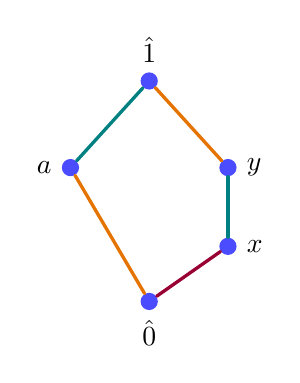
\begin{tikzpicture}[scale=1, line join=round, line cap=round]
  % Styles
    \tikzset{
    v/.style={circle, fill=blue!70, inner sep=2.2pt}, 
    edgea/.style={line width=1.2pt, teal},
    edgeb/.style={line width=1.2pt, orange!90!black},
    edgec/.style={line width=1.2pt, purple!80!black}
   }
  % Nodes
  \node[v,label=above:{$\hat{1}$}]    (top) at (0,1.8) {};
  \node[v,label=left:{$a$}]    (left) at (-1,0.7) {};
  \node[v,label=right:{$y$}]   (right1) at (1,0.7) {};
  \node[v,label=right:{$x$}]   (right2) at (1,-0.3) {};
  \node[v,label=below:{$\hat{0}$}]   (bot) at (0,-1) {}; 
  % Edges (color-coded)
  \draw[edgea] (top)--(left);
  \draw[edgeb] (left)--(bot);
  \draw[edgec] (bot)--(right2);
  \draw[edgea] (right2)--(right1);
  \draw[edgeb] (right1)--(top);
\end{tikzpicture}
\end{minipage}%
\hfill
\begin{minipage}{0.55\textwidth}
   \centering
   % --- M3 Lattice ---
   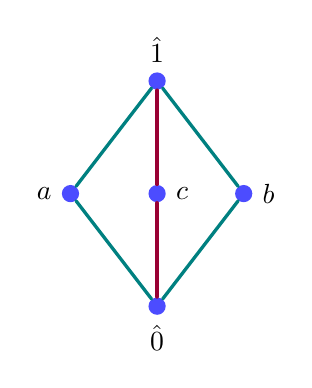
\begin{tikzpicture}[scale=1.1, line join=round, line cap=round]
   % Styles
   \tikzset{
    v/.style={circle, fill=blue!70, inner sep=2.2pt}, 
    edgea/.style={line width=1.2pt, teal},
    edgeb/.style={line width=1.2pt, orange!90!black},
    edgec/.style={line width=1.2pt, purple!80!black}
   }
  % Nodes
  \node[v,label=above:{$\hat{1}$}]    (top) at (0,1.8) {};
  \node[v,label=left:{$a$}]     (left) at (-1,0.5) {};
  \node[v,label=right:{$b$}]    (right) at (1,0.5) {};
  \node[v,label=right:{$c$}]    (mid) at (0,0.5) {};
  \node[v,label=below:{$\hat{0}$}]    (bot) at (0,-0.8) {}; 
  % Edges (color-coded)
  \draw[edgea] (top)--(left)--(bot)--(right)--(top);
  \draw[edgec] (top)--(mid)--(bot);
\end{tikzpicture}
\end{minipage}
\caption{The $N_5$ (left) and the $M_3$ (right) lattices.}\label{FigN5M3S}
\end{figure}
\begin{theorem}[Birkhoff's Characterization Theorem]
A lattice $\mathcal{L}$ is modular if and only if it does not contain a sublattice isomorphic to the pentagon lattice $N_5$.  
Moreover, $\mathcal{L}$ is distributive if and only if it contains no sublattice isomorphic to either the pentagon lattice $N_5$ or the diamond lattice $M_3$.
\end{theorem}
%\begin{theorem}\label{mainmodular}
%    Let \( G \) be a simple graph with the edge ideal \( I(G) \). The $\lcm$-lattice \({\LC}(I(G)) \) is modular if and only if \( G \) contains no induced path of length $3$.
%\end{theorem}

  The following result gives a characterization of modular in the case of hypergraphs.
\begin{theorem}\label{THypermodular} 
    Let $\mathcal{H}$ be a $k$-uniform hypergraph on $n$ vertices with $m>2$ hyperedges, and let 
    \[
    I(\mathcal{H})= (x_{i_1}\cdots x_{i_k} \mid \{i_1,\ldots,i_k\}\in E(\mathcal{H}))
    \]
    denote its corresponding edge ideal, such that at least one of the following conditions holds: 
\begin{itemize}
    \item[(a)] For every hyperedge \( e \in E(\mathcal{H}) \), there exists a vertex \( v_e \in e \) such that \( v_e \notin e' \) for all other hyperedges \( e' \in E(\mathcal{H}) \setminus \{e\} \)
    \item[(b)] \( k = n-1 \), i.e., each hyperedge has cardinality $n-1$.
\end{itemize}
   Then, the $\lcm$-lattice $\LC(I(\mathcal{H}))$ is modular.
\end{theorem}
%
\begin{proof}
%Suppose that $(a)$ does not hold. Then there exists a hyperedge $e$ whose vertices are shared with other hyperedges, say $\{e_{i_1}, \ldots, e_{i_t}\}$. Let 
\[ e_{i_1} \vee \cdots \vee e_{i_t} = m. \] 
%Since $(b)$ also does not hold, we have the following two cases: \\[4pt]

%Case (i): There exists some $e_{i_j}$, for some $j = 1, \ldots, t$, such that 
%\[ |e \cap e_{i_j}| > 1. \]
%Thus, there exists an element $e'$ such that $e_{i_j} \vee e = e' < m$. Then there must exist another hyperedge, say $e_{i_j'}$, such that $e' \wedge e_{i_j'} = \hat{0}$; otherwise, $e' = m$. Therefore, the elements $e, e', e_{i_j'}, m$ together with $\hat{0}$ form a structure isomorphic to $N_5$, which is a contradiction (see \ref{mainpic1} (a)). \\[6pt]

%Case (ii): The hyperedge $e$ differs by exactly one vertex from each of $e_{i_1}, \ldots, e_{i_t}$, and there exists another element, say $e''$, such that 
%\[ |e \cap e''| > 1. \]
%Since $e$ shares all its vertices with $e_{i_j}$, the element $e''$ %is not comparable with $m$. Moreover, we can find another element, %say $m'$, such that $e' < m'$ and $m < m'$, where $m'$ may also be %the maximal element of the poset. In this case, the elements $e, m, %m', e''$ together with $\hat{0}$ form a structure isomorphic to %$N_5$, again a contradiction (see \ref{mainpic1} (b)). \\[6pt]

If $(a)$ holds, then by \ref{Booleanhyper}, $\LC(I(\mathcal{H}))$ is Boolean, and therefore modular.  
If $(b)$ holds, then for each pair of hyperedges $e_i$ and $e_j$, there exists exactly one pair of vertices $v_i$ and $v_j$ such that $v_i \in e_i$ with $v_i \notin e_j$, and $v_j \in e_j$ with $v_j \notin e_i$. Consequently, the join of any two distinct atoms is the maximal element $\hat{1}$, while the meet of any two distinct atoms is $\hat{0}$. Hence, the lattice cannot contain a sublattice isomorphic to $N_5$, and is therefore modular.

\end{proof}
%\begin{figure}[h!]
%\centering
%\begin{minipage}{0.45\textwidth}
%\centering
%\begin{tikzpicture}[
 %   every node/.style={
 %       draw, 
 %       rounded corners, 
 %       minimum size=6mm, 
 %       inner sep=3pt, 
 %       font=\small
 %   }, 
 %   ->, >=Latex, 
  %  scale=0.6, 
  %  transform shape
%]

% ===== Nodes =====
%\node[fill=gray!10] (O) at (0,0) {$\hat{0}$};
%\node[fill=teal!20] (e) at (-2,2) {$e$};
%%\node[fill=orange!20] (ei1) at (0,2) {$e_{i_1}$};
%\node[fill=purple!15] (dots) at (2,2) {$\ldots$};
%\node[fill=purple!20] (eit) at (4,2) {$e_{i_t}$};
%\node[fill=blue!15] (ep) at (-1,4) {$e'$};
%\node[fill=blue!10] (m) at (1,5.5) {$m$};

% ===== Edges =====
%\foreach \x in {e,ei1,dots,eit}{\draw[->, thick] (\x) -- (O);}
%\draw[->, thick] (ep) -- (e);
%\draw[->, thick] (ep) -- (ei1);
%\draw[->, thick] (m) -- (ep);
%%\draw[->, thick] (m) -- (dots);
%\draw[->, thick] (m) -- (eit);

%\end{tikzpicture}
%\\[3pt]
%\textbf{(a)}  Case~(i)%: Lattice with element $e'$ and maximal element $m$.
%\end{minipage}%
%\hfill
%\begin{minipage}{0.45\textwidth}
%\centering
%\begin{tikzpicture}[
 %   every node/.style={
 %       draw,
 %       rounded corners,
 %       minimum size=6mm,
 %       inner sep=3pt,
 %       font=\small
 %   },
 %   ->, >=Latex,
 %   scale=0.6,
 %   transform shape
%]

%% ===== Nodes =====
%\node[fill=gray!10] (O) at (0,0) {$\hat{0}$};
%\node[fill=teal!20]   (a1) at (-2.5,2) {$e$};
%\node[fill=orange!20] (a2) at (-1.3,2) {$e_{i_{1}}$};
%\node[fill=blue!15]   (a4) at (0.2,2) {$\ldots$};
%\node[fill=violet!20] (a5) at (1.6,2) {$e_{i_{t}}$};
%\node[fill=cyan!15]   (a6) at (2.9,2) {$e''$};
%\node[fill=blue!10]   (m1) at (0,4.2) {$m$};
%\node[fill=blue!10]   (m2) at (0,5.8) {$m'$};%

% ===== Edges =====
%\foreach \x in {a1,a2,a4,a5,a6}{\draw[->, thick] (\x) -- (O);}
%\foreach \x in {a1,a2,a4,a5}{\draw[->, thick] (m1) -- (\x);}
%\draw[->, thick] (m2) -- (m1);
%\draw[->, thick] (m2) -- (a6);

%\end{tikzpicture}
%\\[3pt]
%\textbf{(b)}  Case~(ii)%: Lattice extended with elements $e''$ and %$m'$.
%\end{minipage}

%\vspace{4pt}
%\caption{$\lcm$-lattices illustrating the two $N_5$ sublattice.}
%\label{mainpic1}
%\end{figure}
%%%%%%%
%\section{Modular}
%After discussing the results for Boolean $\lcm$-lattices, we now move on to the case of modular $\lcm$-lattices to examine their related properties.
%%%%%%%%%%%%%%%%%%%%%%%%%%%%%%%%%%%%%%%%
The following example illustrates different cases in connection to the above theorem.
\begin{example}\label{exampmodulr}
%Since a lattice $L$ is called \emph{modular} if for all $x,y,z \in L$ with $x \leq z$ we have
%\[
%x \vee (y \wedge z) \;=\; (x \vee y) \wedge z.
%\]
     Let $\mathcal{H}$ be a uniform hypergraph consisting of 3-uniform hyperedges $e_i$. Some cases are computed below to determine whether the corresponding $\lcm$-lattice $\mathcal{L}(I(\mathcal{H}))$ of the edge ideal is modular or not. In particular, we verify whether 
\[
x \vee (y \wedge z) \;=\; (x \vee y) \wedge z,
\]
for all $x, y, z \in \mathcal{L}(\mathcal{H})$ with $x \leq z$ holds, in the given cases.

Case 1: $e_1$ and $e_2$ share a common edge, while $e_2$ and $e_3$ share only a vertex, as shown in \ref{F3} along with the corresponding $\lcm$-lattice.

     
    For $e_1=\{1,2,3\}, e_2= \{2,3,4\}$ and $e_3=\{4,5,6\}$, we have $$I(\mathcal{H})=<x_1x_2x_3, x_2x_3x_4, x_4x_5x_6>,$$  
     Now, let
    \[
      x = x_1x_2x_3, 
      \qquad y = x_4x_5x_6, 
      \qquad z = x_1x_2x_3x_4.
    \]
%%%%%%%%%%%%%%%%%%%%%%%%%%%%%%%%%%%%%%%%
\begin{figure}[h]
     \centering
     \begin{minipage}{0.44\textwidth}
     \centering
     % --- Hypergraph ---
     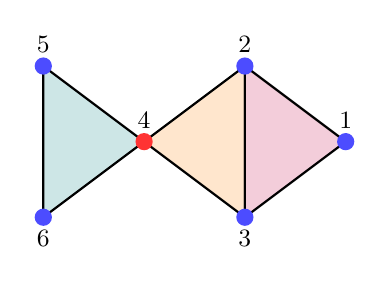
\begin{tikzpicture}[line join=round, line cap=round, scale=0.64]
    % vertex styles
   \tikzset{
    v/.style={circle, fill=blue!70, inner sep=2.2pt},   % vertex
    vc/.style={circle, fill=red!80, inner sep=2.2pt}    % central vertex
     }
  % coordinates
  \coordinate (LT) at (0,1.5);
  \coordinate (LB) at (0,-1.5);
  \coordinate (C)  at (2,0);
  \coordinate (MT) at (4,1.5);
  \coordinate (MB) at (4,-1.5);
  \coordinate (R)  at (6,0);
  % ====== FILLS ======
  \fill[teal!30, opacity=0.65]   (LT) -- (LB) -- (C) -- cycle;   % left triangle
  \fill[orange!30, opacity=0.65] (MT) -- (MB) -- (C) -- cycle;   % middle triangle
  \fill[purple!30, opacity=0.65] (MT) -- (R)  -- (MB) -- cycle;  % right triangle
  % ====== EDGES ======
  \draw[thick] (LT) -- (LB) -- (C) -- cycle;
  \draw[thick] (MT) -- (MB) -- (C) -- cycle;
  \draw[thick] (MT) -- (R) -- (MB) -- cycle;
  % ====== NODES ======
  \node[v]  at (LT) {};
  \node[v]  at (LB) {};
  \node[vc] at (C)  {};
  \node[v]  at (MT) {};
  \node[v]  at (MB) {};
  \node[v]  at (R)  {};
 % ====== VERTEX LABELS (adjust positions if needed) ======
  \node[font=\small, above=1.2pt of LT]  {$5$};
  \node[font=\small, below=1.2pt of LB] {$6$};
  \node[font=\small, above=1.2pt of C]      {$4$};
  \node[font=\small, above=1.2pt of MT]       {$2$};
  \node[font=\small, below=1.2pt of MB] {$3$};
  \node[font=\small, above=1.2pt of R] {$1$};
   \end{tikzpicture}
\end{minipage}%
\hfill
\begin{minipage}{0.55\textwidth}
   \centering
   % --- lcm-lattice ---
   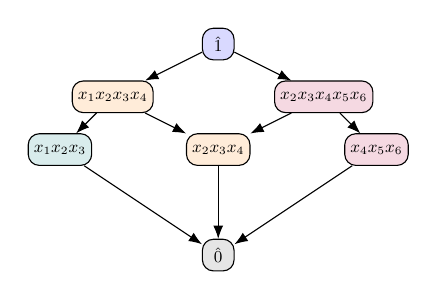
\begin{tikzpicture}[
   every node/.style={draw, rounded corners, minimum size=6mm, inner sep=3pt, font=\small},
  ->, >=Latex, scale=0.67, transform shape]
  % Level 1 (Top)
  \node[fill=blue!15] (A) at (0,4) {$\hat{1}$};
   % Level 2
  \node[fill=orange!15] (B1) at (-2,3) {$x_1x_2x_3x_4$};
  \node[fill=purple!15] (B2) at ( 2,3) {$x_2x_3x_4x_5x_6$};
  % Level 3
  \node[fill=teal!15]   (C1) at (-3,2) {$x_1x_2x_3$};
  \node[fill=orange!15] (C2) at ( 0,2) {$x_2x_3x_4$};
  \node[fill=purple!15] (C3) at ( 3,2) {$x_4x_5x_6$};
  % Level 4 (Bottom)
  \node[fill=gray!20] (O) at (0,0) {$\hat{0}$};
 % Edges
   \draw[->] (A) -- (B1);
  \draw[->] (A) -- (B2);
  \draw[->] (B1) -- (C1);
  \draw[->] (B1) -- (C2);
  \draw[->] (B2) -- (C2);
  \draw[->] (B2) -- (C3);
  \draw[->] (C1) -- (O);
  \draw[->] (C2) -- (O);
  \draw[->] (C3) -- (O);
  \end{tikzpicture}
  \end{minipage}
\caption{A hypergraph with triangular faces and its corresponding $\lcm$-lattice.}\label{F3}
\end{figure}
%%%%%%%%%%%%%%%%%%%%%%%%%%%%%%%%%%%%%%%%
%%%%%%%%%%%%%%%%%%%%%%%%%%%%%%%%%%%%%%%%
    Clearly, $x \leq z$ holds and:
    \begin{eqnarray}
    \nonumber x \vee (y \wedge z) &=& x_1x_2x_3 \vee(x_4x_5x_6\wedge x_1x_2x_3x_4)\\ 
    \nonumber   &=& x_1x_2x_3\vee \hat{0} =x_1x_2x_3,\\
    \nonumber (x \vee y) \wedge z &=& (x_1x_2x_3 \vee x_4x_5x_6)\wedge x_1x_2x_3x_4\\ 
   \nonumber  &=&  \hat{1}\wedge x_1x_2x_3x_4=x_1x_2x_3x_4.
\end{eqnarray}
   Thus, the lattice is \emph{not modular}.\\
    Case 2:
    The four triangles $e_1,e_2,e_3,e_4$ form the faces of a tetrahedron, where each triangular face $e_i$ shares an edge with each of the other three faces.  

    Let $e_1=\{1,2,3\},e_2=\{1,2,4\},e_3=\{1,3,4\},$ and $e_4=\{2,3,4\}$. 
     Then $$I(\mathcal{H})=<x_1x_2x_3, x_1x_2x_4, x_1x_3x_4,x_2x_3x_4>,$$ the corresponding $\lcm$-lattice is shown in \ref{F7}. 
     To verify $x \vee (y \wedge z) \;=\; (x \vee y) \wedge z$, for all $x,y$ and $z$ in $\mathcal{L}(I(\mathcal{H}))$, let
     \[
     x = x_1x_2x_3, 
     \qquad y = x_1x_2x_4, 
     \qquad z = \hat{1}.
     \]
     Clearly, $x \leq z$ holds and: 
\begin{figure}[h]
    \centering
    \begin{minipage}{0.45\textwidth}
    \centering
    % --- Graph (K4 with colored faces + vertex labels) ---
    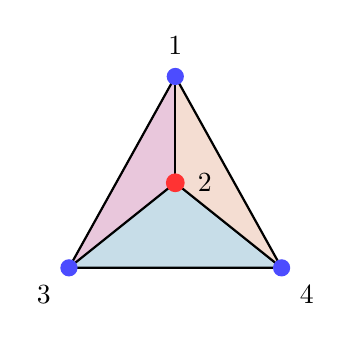
\begin{tikzpicture}[line join=round, line cap=round, scale=1.35]
    % vertex styles
    \tikzset{
    v/.style={circle, fill=blue!70, inner sep=2.2pt},   % outer vertex
   vc/.style={circle, fill=red!80, inner sep=2.4pt},   % central vertex
   }
   % coordinates
   \coordinate (A) at (-1,-0.6);
   \coordinate (B) at ( 1,-0.6);
   \coordinate (C) at (0,1.2);
   \coordinate (D) at (0,0.2); % central vertex
   % shaded triangles (faces = atoms)
   \fill[blue!20, opacity=0.7]   (A)--(B)--(C)--cycle;  % 123
   \fill[teal!25, opacity=0.7]   (A)--(B)--(D)--cycle;  % 124
   \fill[orange!25, opacity=0.7] (B)--(C)--(D)--cycle;  % 234
   \fill[purple!25, opacity=0.7] (C)--(A)--(D)--cycle;  % 134
   % edges
   \draw[thick] (A)--(B)--(C)--cycle;  % outer triangle
   \draw[thick] (A)--(D);
   \draw[thick] (B)--(D);
   \draw[thick] (C)--(D);
   % vertices
  \node[v]  (nA) at (A) {};
  \node[v]  (nB) at (B) {};
  \node[v]  (nC) at (C) {};
  \node[vc] (nD) at (D) {};
  % labels for vertices
  \node[below left=1pt of nA] {$3$};
  \node[below right=1pt of nB] {$4$};
  \node[above=1pt of nC] {$1$};
  \node[right=1pt of nD] {$2$};
  \end{tikzpicture}
\vspace{0.2cm}
\end{minipage}%
\hfill
\begin{minipage}{0.55\textwidth}
   \centering
  % --- Poset ---
   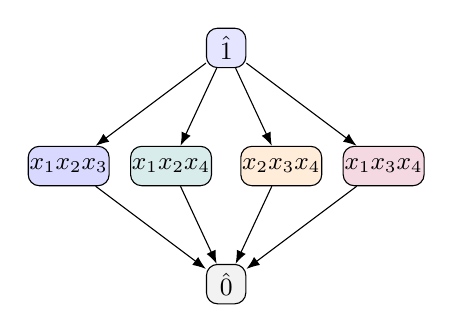
\begin{tikzpicture}[scale=1, every node/.style={draw, rounded corners, minimum size=5mm, inner sep=0.5pt, font=\small}, ->, >=Latex]
   % Top
   \node[fill=blue!10] (T) at (0,3.5) {$\hat{1}$};
   % Middle level = atoms (light pastel fills)
   \node[fill=blue!15]   (A) at (-2,2) {$x_1x_2x_3$};
   \node[fill=teal!15]   (B) at (-0.7,2) {$x_1x_2x_4$};
   \node[fill=orange!15] (C) at (0.7,2) {$x_2x_3x_4$};
   \node[fill=purple!15] (D) at (2,2) {$x_1x_3x_4$};
   % Bottom
   \node[fill=gray!10] (O) at (0,0.5) {$\hat{0}$};
   % Edges
   \draw[->] (T)--(A);
   \draw[->] (T)--(B);
   \draw[->] (T)--(C);
   \draw[->] (T)--(D);
   \draw[->] (A)--(O);
   \draw[->] (B)--(O);
   \draw[->] (C)--(O);
   \draw[->] (D)--(O);
   \end{tikzpicture}
\vspace{0.2cm}
\end{minipage}
\caption{The hypergraph with triangular faces, and its corresponding $\lcm$- lattice}\label{F7}
\end{figure}
%%%%%%%%%%%%%%%%%%%%%%%%%%%%%%
    \begin{eqnarray}
     \nonumber x \vee (y \wedge z) &=& x_1x_2x_3 \vee(x_2x_3x_4\wedge \hat{1})\\ 
     \nonumber   &=& x_1x_2x_3\vee x_2x_3x_4 =\hat{1},\\
     \nonumber (x \vee y) \wedge z &=& (x_1x_2x_3 \vee x_2x_3x_4)\wedge \hat{1}\\ 
     \nonumber  &=&  \hat{1}\wedge \hat{1}=\hat{1}.
     \end{eqnarray}
     This lattice has just two levels of atoms under the top and one bottom, it does not contain $N_5$ as a sublattice. Thus, the lattice is modular for any $x,y$, and $z$.
\end{example}

%\textbf{Observations:}\\

%    \item  A unique complemented non distributive lattice is necessarily non atomic and non modular.
   % \item Boolean lattice $\Rightarrow$ Complemented lattice $\Rightarrow$ Atomic lattice.
   % \item Complemented lattice is unique iff it is Boolean lattice.
  

   % A lattice fails to be complemented if it contains subgraphs like:

    %\item A chain of length 3 (no complements for middle).
    %\item some middle elements the diamond lattice $M_3$ have no complements.
   
   %A finite, atomic, distributive lattice is Boolean becasue it is a finite, atomic, uniquely complemented lattice.

   % The paper is organized as follows: the succeeding section articulates the preliminary definitions,  section $2$ contains principal results, and then in section $3$, concludes with future work. 


%The lcm-lattice of a monomial ideal is always atomic, with atoms corresponding to the minimal generators of the ideal.
%\begin{theorem}
 % \textcolor{red}{  Let $G$ be a graph and $I(G)$ be its edge ideal then $G$ is atomic iff G is path of length $2$ only or not contains a path length $3$ with $2$ end leaves.}
%\end{theorem}

%\begin{proof}
%Suppose that $G$ contains a path of length $3$. Then \[I(G) = (x_1 x_2,\, x_2 x_3,\, x_3 x_4).\]In the LCM-lattice $\LC(I(G))$, the element $x_1 x_2 x_3 x_4$ cannot be expressed as the join of atoms, since\[\mathrm{lcm}(x_1 x_2,\, x_2 x_3) = x_1 x_2 x_3, \quad \mathrm{lcm}(x_2 x_3,\, x_3 x_4) = x_2 x_3 x_4,\]and $\mathrm{lcm}(x_1 x_2 x_3,\, x_2 x_3 x_4) = x_1 x_2 x_3 x_4$ not generated by smaller atomic joins. Hence $\LC(I(G))$ is not atomic.Conversely, assume that $G$ does not contain such a path. Then every induced subgraph of $G$ consists of edges of a path of length $2$. As,$\LC (I(G))$ is isomorphic to a Boolean lattice iff \( G \) contains no path of length $3$. So, every element of $\LC(I(G))$ is the join of its generating edges (atoms), and thus $\LC(I(G))$ is atomic.
%\end{proof}
\subsection{Hypergraphs and Complemented Lattices}
    

\begin{definition}
    If $L$ is a bounded lattice then we say that $y \in L$ is a complement of $x \in L$ if $\exists ~ \hat{0}, \hat{1} $ such that  $x \wedge y = 0$ and $x \vee y = 1.$ In this case, we say that $x$ is a complemented element of $L$. Clearly, every complement of a complemented element is itself complemented. A lattice $L$ is a complemented lattice if every element of $L$ is complemented.
\end{definition} 
%\begin{example}
 %    $D_6= \{1, 2, 3, 6\}$ is a complemented lattice. 
%\end{example}  
 

%\begin{definition}
 %   A lattice in which every element has exactly one complement is called a uniquely complemented lattice.
%\end{definition}

%\begin{definition}\label{DefHyperG}
%A \emph{$k$-uniform hypergraph} is a hypergraph $\mathcal{H} = (V, E)$, where $V$ is the vertex set and $E$ is the set of hyperedges, such that every hyperedge $e \in E$ contains exactly $k$ distinct vertices; that is, $|e| = k$ for all $e \in E$.
%\end{definition}
 
%\section{Results and Discussion}\label{sec2}
%   In this section, we present the main results, along with few examples. 

  
%\begin{remark}
  %   Let $\H$ be a uniform hypergraph and $A,B \subseteq E(\H)$ be two subsets from the edge set of $\H$. In the Theorem \ref{Booleanhyper}, the statement $(b)$ is equivalent to the following statement:\\
   %  if ${\cup}_{e \in B}e =\cup_{e\in A}e $, then $A=B$. The statement is true using the arguments given in the proof of the above theorem.
%\end{remark}
\begin{theorem}
Let $G$ be a connected graph and $I(G)$ be its edge ideal. If $G$ does not contain a path
\[
\{x_1,x_2,x_3,x_4\},
\]
such that $x_1$ and $x_4$ have degree $1$, then $\LC(I(G))$ is complemented.
\end{theorem}\begin{proof}
 %     Let $\mathcal{L}(I(G)) $ be complemented. Suppose on contrary, $G$ contain a paths, say, $$\{x_1,x_2, \ldots, x_4\}$$ such that $x_1$ and $x_4$ have degree $1$.  Then consider the element $u=x_2x_3 \in \mathcal{L}(I(G))$. Then $u$ does not contain a complement in $\mathcal{L}(I(G))$, because a complement $u'$ of $u$ must contain $x_1$ and $x_4$. However, to take $x_1$ and $x_4$ in $u'$, we must have $x_2$ and $x_3$ both in $u'$. Thus $\mathcal{L}(I(G)) $ is not complemented, a contradiction.

     Let $G$ does not contain any path of edges, say, $\{x_1,x_2\},$ $\{x_2,x_3\}, \{x_{3},x_4\}$ such that $x_1$ and $x_4$ have degree $1$. Let $u \in \mathcal{L}(I(G))$, with $\supp(u) =A\subseteq V(G)$, such that there exist a subset $E' \subset E(G)$ with $A=\cup_{e\in E'} e.$ Set $B =V(G) \setminus A $ and 
     $$B'=\{u \in B| u \text{ is not connected to another vertex in } B\}.$$ 
     Also, let $$C= B\setminus B' \cup \{\{u,w\}\in E(G) | u\in B'\}.$$
     Now there are two cases:

     Case $(i):$ $B'=\emptyset $. In this case, there exist $v \in \mathcal{L}(I(G))$ such that $\supp(v)=B=C$. It is easy to see, $v$ is the complement of $u$ in $\mathcal{L}(I(G))$.

     Case $(ii):$ $B'\not=\emptyset $. Since all vertices in $B'$ has degree $1$, then by supposition, as $G$ does not contain a paths, say, $\{x_1,x_2, \ldots, x_4\}$ such that $x_1$ and $x_4$ have degree $1$. Therefore, there exist $v \in \mathcal{L}(I(G))$  such that $\supp(v)=C$. But then we have $u \wedge v = \emptyset$, because there does not exist any common edge, between $x_2$ and $x_3$. Moreover, since $A \cup C = V(G)$, thus $v$ is the complement of $u$ in $\mathcal{L}$.
\end{proof}



\begin{theorem}
     Let $H$ be a $k$-uniform hypergraph and $I(H)$ its edge ideal. Then $\LC(I(H))$ is complemented if and only if $H$ does not contain a triplet of hyperedges $\{e_1, e_2, e_3\}$ such that $e_1$ and $e_3$ do not share vertices with any other hyperedge except $e_2$, where 
\[
e_1 \cap e_2 \neq \emptyset, \quad e_2 \cap e_3 \neq \emptyset, \quad \text{and} \quad |\,\{e_1, e_3\} \cap e_2\,| = |e_2|.
\]
\end{theorem}
\begin{proof}
    Let $\LC(I(H))$ be complemented and suppose that on contrary there exists a triplet of hyperedges, say $\{e_1, e_2. e_3\}$ such that it satisfies the given conditions. Now, let $u=e_2 \in \LC(I(H))$ be an element, then the complement $v$ of $u$ must contain $e_1\setminus e_2$ and $e_3\setminus e_2$. Then since $e_1 \cap e_2 \neq \emptyset, \quad e_2 \cap e_3 \neq \emptyset, \quad \text{and} \quad |\,\{e_1, e_3\} \cap e_2\,| = |e_2|$, this implies $e_2$ must belong to $v$, which contradics the definition of complement of an element. Therefore, $\LC(I(H))$ is not complemented, a contradiction.

    Conversely, there does not exist any triplet of hyperedges, say $\{e_1, e_2. e_3\}$ such that it satisfies the given conditions. Let $u$ be an element of $\LC(I(H))$ such that $A = \cup_{e\in u}e$ and let $B=V(H)\setminus A$. Now let 
    $$B'=\{u \in B \,\,|\,\, u \text{ is not connected to another vertex in } B\}.$$ 
    Also, let $$C= B\setminus B' \cup \{\{u,w\}\in E(G) | u\in B'\}.$$
    Now there are two cases:

    Case $(i):$ $B'=\emptyset $. In this case, there exist $v \in \mathcal{L}(I(G))$ such that $\supp(v)=B=C$. It is easy to see, $v$ is the complement of $u$ in $\mathcal{L}(I(G))$.

    Case $(ii):$ $B'\not=\emptyset $. Since all vertices in $B'$ do not share any vertex with any other vertex in B, then by supposition, as $G$ does not contain a paths, say, $\{x_1,x_2, \ldots, x_4\}$ such that $x_1$ and $x_4$ have degree $1$. Therefore, there exist $v \in \mathcal{L}(I(G))$  such that $\supp(v)=C$. But then we have $u \wedge v = \emptyset$, because there does not exist any common edge, between $x_2$ and $x_3$. Moreover, since $A \cup C = V(G)$, thus $v$ is the complement of $u$ in $\mathcal{L}$.

\begin{example}
Consider the lattice with elements
\[
\{0,\;12,\;13,\;24,\;123,\;124,\;1234\}.
\]

\begin{figure}[h]
    \centering
    \begin{minipage}{0.45\textwidth}
        \centering
        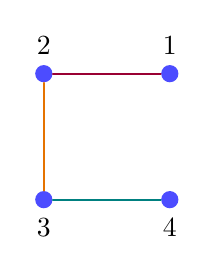
\begin{tikzpicture}[scale=0.8, line join=round, line cap=round]
            \tikzset{
                v/.style={
                    circle,
                    fill=blue!70,
                    inner sep=2.2pt,
                    font=\small,
                    text=white
                }
            }

            \node[v,label=below:{$4$}] (v1) at (2,0) {};
            \node[v,label=below:{$3$}] (v2) at (0,0) {};
            \node[v,label=above:{$2$}] (v3) at (0,2) {};
            \node[v,label=above:{$1$}] (v4) at (2,2) {};

            \draw[teal, thick] (v1)--(v2);
            \draw[orange!90!black, thick] (v2)--(v3);
            \draw[purple!80!black, thick] (v3)--(v4);
        \end{tikzpicture}
        \vspace{0.2cm}
    \end{minipage}%
    \hfill
    \begin{minipage}{0.45\textwidth}
        \centering
        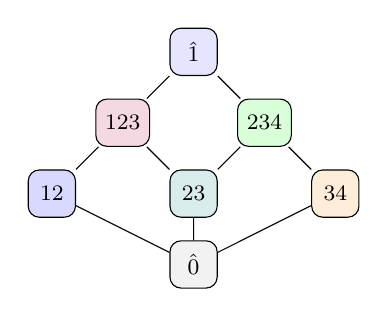
\begin{tikzpicture}[
            every node/.style={
                rounded corners,
                draw,
                minimum size=6mm,
                font=\footnotesize
            },
            scale=0.6
        ]

            \node[fill=gray!10] (0) at (0,0) {$\hat{0}$};

            \node[fill=blue!15] (12) at (-3,1.5) {$12$};
            \node[fill=teal!15] (23) at (0,1.5) {$23$};
            \node[fill=orange!15] (34) at (3,1.5) {$34$};

            \node[fill=purple!15] (123) at (-1.5,3) {$123$};
            \node[fill=green!15] (234) at (1.5,3) {$234$};

            \node[fill=blue!10] (1) at (0,4.5) {$\hat{1}$};

            \draw (0)--(12) (0)--(23) (0)--(34);
            \draw (12)--(123) (23)--(123);
            \draw (23)--(234) (34)--(234);
            \draw (123)--(1) (234)--(1);

        \end{tikzpicture}
    \end{minipage}

    \caption{The path graph $P_4$ and its corresponding $\lcm$-lattice.}
    \label{F5}
\end{figure}

As illustrated in \ref{F5}, consider the $\lcm$-lattice
\[
L=\{0,\;12,\;13,\;24,\;123,\;124,\;1234\}.
\]
The elements $12$ and $34$ are complements of each other, since
\[
12\wedge 34=0
\qquad\text{and}\qquad
12\vee 34=1234.
\]
However, the element $23$ has no complement in $L$, since its complement would be $14$, which is not an element of the lattice.
Likewise, $123$ would require $4$ as a complement, while $234$ would
require $1$; neither $4$ nor $1$ belongs to $L$.

Hence, not every element of $L$ has a complement. Therefore, the
$\lcm$-lattice $L$ is not complemented.
\end{example}

\end{proof}

%\begin{lemma}
 %    lcm$(I_{P_n})$ is not complemented  as no contains a path of length 3
%\end{lemma}
%\begin{proof}
%\end{proof}

\begin{definition}
    A lattice $L$ is a \emph{relatively complemented lattice} if every interval $[x, y]$(viewed as a sublattice) of $L$ is complemented. 
\end{definition}

\begin{remark}
    In a distributive lattice, all complements and relatively complements of poset are unique. 
\end{remark}
%\begin{theorem}\label{asd}Let \( G = (V, E) \) be a simple graph, and let \( I(G) = (x_i x_j \mid \{i, j\} \in E) \) be its edge ideal with \( \LC(I(G)) \) to be its LCM-lattice. Then the following are equivalent:\begin{itemize} \item[a)] $\LC (I(G))$ is isomorphic to a Boolean lattice\item[b)] \( G \) contains no path of length $3$\item[c)] each edge of \( G \) can be uniquely identified by a single vertex.\end{itemize}  \end{theorem}

\begin{theorem}
     Let $G$ be a connected graph and $I(G)$ be its edge ideal, then $lcm(I(G))$ is \emph{relatively complemented} if and only if there exists no induced subgraph $G|_W$ on the vertex set $W \subseteq V$ such that ${G|_W}$ is of path length $ \geq 3$.
\end{theorem}
\begin{proof}
     %  Contrary suppose that there exists a path of length greater than equal 3. Suppose that we have a path $\{x_1,x_2\},\{x_2,x_3\},\{x_3,x_4\},\ldots,\{x_{i-1},x_i\}$ such that $d_i=1$ and $d_{i-1}=2$ then $x_1,x_2,\ldots, x_{i-2}$ will not have a complement because its complement must contains $x_{i-1}$ and $x_i$ that do not exist in the $\lcm$ lattice of this path graph.  So there exists a chain having $x_1,x_2,\ldots, x_{i-2} \longrightarrow x_1,x_2,\ldots, x_{i-1} \longrightarrow x_1,x_2,\ldots, x_{i}$ but here we can not find an element/ atom $x_{i-1}x_i$. So our assumption for being length greater than equal 3 to be complemented is wrong. which implies that a graph with length less than equal 3 is always relatively complemented.\\
%
     %   \textbf{Conversally,} suppose that for a connected graph G and its edge ideal $I(G)$, $lcm(I(G))$ is relatively complemented. We need to prove that there exists no induced subgraph $G| _w$
    %   on the vertex set $W \subseteq V$ such that ${G| _w}$ is a path of length $i \geq 3$.\\
%
    %    Let $u \in \mathcal{L}=\lcm (I(G))$. Let $\supp(u) =A\subseteq V(G)$, such that $A=\cup_{e\in E' \subset E(G)} e.$ Set $B =V(G) \setminus A $ and $A \subset B $  such that chain $x_{i-1}$ %\subset
    %    is properly contained in the chain of elements $x_i$, for all $i$. Then we have two cases:\\
%
%
    % Case $(i):$ If we will choose an interval $[x_1,x_n]$ such that $x_j \in$  $[x_1,x_n]$ such that  then each atom will contain $x_1,x_n$ a path having a shape of  
   % Case $(ii):$

%%%%%%%%%%%%%%%%%%%%%%%%%%%%%%%%
%
    %Let $G$ be a connected graph and $I(G)$ be its edge ideal then 
     Suppose that $\lcm(I(G))$ is relatively complemented. 
To the contrary, assume that there exists an induced subgraph $W \subseteq V$ having a path of length $3$, where 
$W = \{x_1x_2,\, x_2x_3,\, x_3x_4\}$. 
Then, the interval 
\[
[a,\, \{x_1x_2x_3x_4\}]
\]
is not complemented for $a \in \{x_1x_2,\, x_3x_4\}$. \\[4pt]
Conversely, suppose that there exists no induced subgraph of path length $3$. 
This means that $G$ has a maximum induced path of length two. 
We now show that $\lcm(I(G))$ is relatively complemented. 
Since the $\lcm$-lattice of a graph having path length at most $2$ is Boolean, and every Boolean lattice is relatively complemented, we conclude that $\lcm(I(G))$ is relatively complemented.

\end{proof}
%\textbf{Remarks:}
%\begin{itemize}
%    \item Relatively Complemented lattice is equal to a Complemented lattice iff it is Modular lattice.
%
%   \item Complemented lattice $\Rightarrow$ Relatively Complemented lattice.
%
%   \item Relatively Complemented lattice $\not\Rightarrow$ Complemented lattice.
%
%    \item Lower Complemented lattice $\Rightarrow$ Relatively Lower Complemented lattice.
%\end{itemize}
%
%The following relations summarize the hierarchy among complemented, relatively complemented, and modular lattices:
%
%\begin{itemize}
%    \item Every complemented modular lattice is relatively complemented.
%
%    \item Every bounded relatively complemented lattice is complemented.
%
%    \item A complemented lattice need not be relatively complemented.
%
%    \item A relatively complemented lattice need not be modular.
%
%    \item Every lower complemented lattice is relatively lower complemented.
%\end{itemize}
%
%
%\subsection*{Locally Relatively Complelmented Lattice }
%\begin{definition}
 %   A lattice $L$ is called locally relatively complemented (LRC) if every finite interval in $L$ is relatively complemented i.e, for every pair $a\leq b$ in $L$, the interval $[a,b]$ forms a relatively complemented lattice.
%\end{definition}
%\begin{theorem}
%    Let G be a graph then
%\end{theorem}
%\begin{proof}
%\end{proof}
\subsection{Product of $\lcm$-Lattices}
We start with following basic property of the $\lcm$-lattices.
\begin{definition}
    %\textbf{Product of Lattices:}  
    Given two lattices $L_1$ and $L_2$, then the product of lattices $L_1 \times L_2$ forms a lattice in a natural way. The partial order is defined by:
\(
(x_1, y_1) \leq (x_2, y_2) 
\quad \text{if and only if} \quad
x_1 \leq x_2 \ \text{in } L_1 \ \text{and}\ y_1 \leq y_2 \ \text{in } L_2.
\)
\end{definition}

\begin{proposition}
     Let $L_1, \ldots, L_r$ be the lattices then $L_1 \times L_2 \ldots \times L_r$ be complemented if and only if $L_1, \ldots, L_r$ be complemented.
\end{proposition}
%\begin{proof}
%     Suppose that $L_1, \ldots, L_r$ be complemented for all $x_i \in L_i$,
%     There exists some  $ x_{i} ^{'} \in L_i $
%     where  $x_{i} ^{'}$  be the complement %that is also not unique.
%     such that
%     $x_i  \vee x_{i} ^{'} = \hat{1}$ and   $x_i  \wedge x_{i} ^{'}=\hat{0}$\\
     %$\Leftrightarrow$ 
%     $\Leftrightarrow$  Now, let $u_i=(x_1,x_2, \ldots,x_k ) \in L_1 \times L_2 \ldots \times L_r$ 
 %     for all
 %     $x_i \in L_i$ then there exists some complement of
 %     $u^{'} _i$ of $u_i$ where
 %    $u_i^{'}=(x_1^{'}, x_2^{'} , 
 %    \ldots,x_k^{'} ) \in L_1 \times L_2 \ldots \times L_r$.\\ such that 
 %     $  u_i \vee u^{'} _i= \hat{1}$  and 
 %     $u_i \wedge u^{'} _i= \hat{0}$
%\end{proof}

%\begin{proposition}
%Let $L_1, L_2, \dots, L_r$ $(r \geq 1)$ be bounded lattices.  
%The direct product lattice $L = L_1 \times L_2 \times \cdots %\times L_r$ (with componentwise operations and order) is complemented if and only if each $L_i$ is complemented.
%\end{proposition}
\begin{proof}
$(\Rightarrow)$  
Let $L=L_1 \times L_2 \times \cdots \times L_r$ be complemented. Let $x_i \in L_i$ and consider the element $a = (0_1, \dots, 0_{i-1}, x_i, 0_{i+1}, \dots, 0_r) \in L$.  
Since $L$ is complemented, there exists $a' = (y_1, \dots, y_r) \in L$ such that  
$$a \vee a' = 1_L \quad \text{and} \quad a \wedge a' = 0_L.$$  
Now the $i$-th component gives  
$$x_i \vee y_i = 1_{L_i} \quad \text{and} \quad x_i \wedge y_i = 0_{L_i}.$$  
Thus $y_i$ is a complement of $x_i$ in $L_i$. Since $x_i$ was arbitrary, $L_i$ is complemented.

$(\Leftarrow)$  
Now let $L_i$ is complemented for all $i$. Let $u = (x_1, x_2, \dots, x_r) \in L$.  
Now for each $x_i\in L_i$, there exist a complement $x_i' \in L_i$ such that:  
$$x_i \vee x_i' = 1_{L_i} \quad \text{and} \quad x_i \wedge x_i' = 0_{L_i}.$$  
Set $u' = (x_1', x_2', \dots, x_r') \in L$.  
Then from above:  
$$u \vee u' = (x_1 \vee x_1', \dots, x_r \vee x_r') = (1_{L_1}, \dots, 1_{L_r}) = 1_L$$  
and  
$$u \wedge u' = (x_1 \wedge x_1', \dots, x_r \wedge x_r') = (0_{L_1}, \dots, 0_{L_r}) = 0_L.$$  
Therefore $u'$ is a complement of $u$ in $L$. 

\end{proof}

\subsection{Impact of Polarization on $\lcm$-lattices}\label{subsec2}
In the above discussion, we have considered it $I$ to be a square-free monomial ideal. To extend these results to the case of a general monomial ideal $I$ in the polynomial ring $S$, we use the concept of \emph{polarization}, as defined below. In particular, we aim to show that the $\lcm$-lattice of $I$ and that of its polarization $I^{p}$ are isomorphic. Consequently, all the above results will also hold for any monomial ideal $I$.

\begin{definition}%[Polarization of a Monomial Ideal]

    Let $S = \mathbb{K}[x_1, x_2, \ldots, x_n]$ be a polynomial ring over a field $\mathbb{K}$, and let 
   \[
    I = (u_1, u_2, \ldots, u_m) \subseteq S
   \] 
    be a monomial ideal, where each $u_j = x_1^{a_{1j}} x_2^{a_{2j}} \cdots x_n^{a_{nj}}$ is a monomial in $S$. The \emph{polarization} of $I$, denoted $I^{p}$, is a square-free monomial ideal obtained in a larger polynomial ring 
    \[
    S^{p} = \mathbb{K}[x_{i1}, x_{i2}, \ldots, x_{i a_i} \mid 1 \leq i \leq n],
    \] 
     where $a_i = \max_j \{a_{ij}\}$. Each monomial $u_j$ is replaced by the square-free monomial
    \[
     u_j^{p} = \prod_{i=1}^n \prod_{k=1}^{a_{ij}} x_{ik}.
    \]
    Then, 
    \[
     I^{p} = (u_1^{p}, u_2^{p}, \ldots, u_m^{p}).
    \]
\end{definition}
%
\begin{example}
    Consider the polynomial ring $S = \mathbb{K}[x_1, x_2]$ and the monomial ideal
   \[
    I = (x_1^2 x_2, \; x_2^3).
    \]
    To polarize, we introduce new variables $x_{11}, x_{12}$ for $x_1^2$ and $x_{21}, x_{22}, x_{23}$ for $x_2^3$. Thus, in 
    \[
     S^{p} = \mathbb{K}[x_{11}, x_{12}, x_{21}, x_{22}, x_{23}],
    \]
    the polarized ideal is
    \[
    I^{p} = (x_{11}x_{12}x_{21}, \; x_{21}x_{22}x_{23}).
    \]
    Here, $I^{p}$ is square-free, and it preserves many algebraic properties of $I$.
    So, for $I$, polarization gives $ I^{p}$, preserving the $\lcm$-lattice structure.
\end{example}   
 The following result shows that polarization preserves the $\lcm$-lattice isomorphism between monomial and square-free ideals. This enables us to extend our characterizations of Boolean and modular properties to any monomial ideal.

\begin{lemma}\label{Tpolarization}
    Let \( I \subset S = \mathbb{K}[x_1, \ldots, x_n] \) be a monomial ideal and let \( I^p \) denote its polarization. Let \( \mathcal{L}(I) \) and \( \mathcal{L}(I^p) \) be the $\lcm$-lattices of \( I \) and \( I^p \), respectively. Then,
    \[
    \mathcal{L}(I) \cong \mathcal{L}(I^p).
    \]
\end{lemma}

\begin{proof}
    The $\lcm$-lattice of a monomial ideal is atomic, and two monomials are equal if and only if their polarizations are equal. It suffices to show that the polarization of the join of two monomials equals the join of their polarizations; that is $(m_1 \vee m_2)^p = m_1^p \vee m_2^p$.
    %%%%%%%%%%%%%%%%%%%%%%%%%%%%%
    Let \( m_1 = x_1^{\alpha_1} \cdots x_n^{\alpha_n} \) and \( m_2 = x_1^{\beta_1} \cdots x_n^{\beta_n} \). Then,
    \[
    m_1 \vee m_2 = x_1^{\max(\alpha_1, \beta_1)} \cdots x_n^{\max(\alpha_n, \beta_n)}.
    \]
    The polarization of \( m_1 \) and \( m_2 \) are given by:
    \[
    m_1^p = \prod_{i=1}^n \prod_{j=1}^{\alpha_i} x_{ij}, \quad
    m_2^p = \prod_{i=1}^n \prod_{j=1}^{\beta_i} x_{ij}.
    \]
    Therefore,
    \[
    m_1^p \vee m_2^p = \prod_{i=1}^n \prod_{j=1}^{\max(\alpha_i, \beta_i)} x_{ij},
    \]
    which is exactly the polarization of \( m_1 \vee m_2 \). Hence,
    \[
    (m_1 \vee m_2)^p = m_1^p \vee m_2^p.
    \]
    This shows that the $\lcm$-lattices \( \mathcal{L}(I) \) and \( \mathcal{L}(I^p) \) are isomorphic.
\end{proof}

%\begin{definition}
 %    A lattice $L$ is called \emph{strongly complemented} if for every $x \in L$, 
 %    there exist elements $y, z \in L$ such that $y$ is a meet of coatoms and $z$ is a join of atoms, with 
 %    \[
 %     x \vee y \;=\; x \vee z \;=\; 1, 
 %     \quad \text{and} \quad 
  %    x \wedge y \;=\; x \wedge z \;=\; 0.
  %    \]
%\end{definition}
%\begin{remark}
%    Every strongly complemented lattice is complemented, but the converse does not hold in general.
%\end{remark} 
 %   Complements of each element form a sublattice for strongly complemented lattice. Every Boolean lcm-lattice for example, $I = (x_1,\ldots,x_n)$ is strongly complemented. However, in general, lcm-lattices are complemented but not strongly complemented.\\
%\textbf{Remarks:}
%\begin{enumerate}
 % \item Every strongly complemented lattice is (in particular) a complemented lattice.
 % \item Every bounded relatively complemented lattice is complemented.
 % \item A complemented lattice need not be relatively complemented (nor strongly complemented) in general; additional hypotheses (e.g. modularity) are required for the converse.
%\end{enumerate}
%%%%%%%%%%%%%%%%%%

%\section*{Acknowledgements}

%T%he authors sincerely thank Volkmar Welker for proposing this problem and for his valuable discussions on its solution. The first author is supported by the International Mathematical Usnion through the Graduate Research Assistantships in Developing Countries (GRAID) Program.

%\section*{Funding}
%The first author has been sponosored by International Mathematical Union, under its GRAID program.

%
\begin{thebibliography}{xxx}

\bibitem{BirkhoffG1967} Birkhoff, G. (1967). Lattice theory, vol. XXV. In American Mathematical Society Colloquium Publications, Providence, RI.

\bibitem{DaveyPristley2002} Davey, B. A., \& Priestley, H. A. (2002). Introduction to lattices and order. Cambridge University Press.

\bibitem{DorangMc2025} Dorang, M., \& McCullough, J. (2025). Properties of LCM lattices of monomial ideals. arXiv preprint arXiv:2505.08722.

\bibitem{DorangMT2025} Dorang, M. T. (2025). Characterizations of edge ideals via LCM lattices (Master's thesis, Iowa State University).

\bibitem{sara} Faridi, S. (2019). Lattice complements and the subadditivity of syzygies of simplicial forests. Journal/Conference, 535-546.

\bibitem{GhoshPaulos2024} Ghosh, D., Gyori, E., Nagy-Gyorgy, J., Paulos, A., Xiao, C., \& Zamora, O. (2024). Book free 3-uniform hypergraphs. Discrete Mathematics, 347(3), 113828.

\bibitem{HerzogHibi2011} Herzog, J., \& Hibi, T. (2011). Monomial ideals. In Monomial ideals (pp. 3-22). London: Springer London.

\bibitem{KIMURATERAI} Kimura, K., Rinaldo, G., \& Terai, N. (2012). Arithmetical rank of squarefree monomial ideals generated by five elements or with arithmetic degree four. Communications in Algebra, 40(11), 4147-4170.

\bibitem{LinMcCullough2013} Lin, K. N., \& McCullough, J. (2013). Hypergraphs and regularity of square-free monomial ideals. International Journal of Algebra and Computation, 23(07), 1573-1590.

\bibitem{KUEISONJA2022} Lin, K. N., \& Mapes, S. (2022). Lattices and hypergraphs associated to square-free monomial ideals. Communications in Algebra, 50(11), 4710-4724.

\bibitem{StanleyRP2011} Stanley, R. P. (2011). Enumerative combinatorics volume 1 second edition. Cambridge Studies in Advanced Mathematics.

\bibitem{WelkerPV1999} Welker, V. (1999). The LCM lattice in monomial resolutions. Mathematical Research Letters, 6, 521-532.



\end{thebibliography}
\end{document}

%
%
 % A binary relation $\leq$ on a non empty set $P$ is called a \emph{partial order} if it is reflexive, antisymmetric, and transitive
  % A \emph{binary relation} on a non-empty set $E$ is defined as a subset $R$ of the Cartesian product: \[E \times E = \{(x, y) \mid x, y \in E\}.\]
%
   % A \emph{meet-semilattice} is a poset in which every pair of elements has a greatest lower bound (meet). Similarly, a \emph{join-semilattice} is a poset in which every pair of elements has a least upper bound (join). 
   %
   %A \emph{lattice} is an ordered set $(E, \leq)$ that, with respect to its order, is both a meet-semilattice and a join-semilattice.
%
   \begin{remark}
     Every chain is a meet semilattice in which $x \wedge   y = min\{x, y\}.$
\end{remark}


%%%%%%%%%%%%%%%%%%%%%%%%%%%%%%%%%%%%%%%%%%%%%%%%%%%%%%%%%%%%%%%%%%%%%%%%%
\\paper 01\\
%%%%%%%%%%%%%%%%%%%%%%%%%%%%%%%%%%%%%%%%%%%%%%%%%%%%%%%%%%%%%%%%%%%%%%%%%%%%%%%%%%%%






\begin{definition}
      Suppose $V=F_q^n$ be a finite n dimensional vector space and consider $\Omega$  and build a \textbf{collection of all simplicial complex} 
      $\Omega=\{U| U$ is a subspace of $V\}$ with property\\ 
      $\Delta_{V}=\{A$ is subspace of $\Omega |  \exists $  basis $B$ of $V$ with $B \bigcap  U$ is basis for $U$, for all $U \in  A\}$  
\end{definition}
%%%%%%%%%%%%%%%
\begin{definition}
    For \textbf{minimal non-faces}, If any of these subsets do not form a face of the complex, then they are minimal non-faces of complex. 
\end{definition}
%%%%%%%%%%%%%%%%%%
\section{Complete Intersection}
    Well known result (Guess)
\begin{lemma}
     Let $I=(m_1,\ldots,m_r)$ be a square free monomial ideal then is a complete intersection iff $gcd(m_1,m_r)=1$\\
\end{lemma}
\begin{proof}
    \textcolor{red}{\textbf{Proof 01}}
\end{proof}
\bigskip
\begin{lemma}
     If $m_{1},m_{2}, m_{3}  \in lcm(I)$ and $m_{1}/m_{2}$ then $lcm(m_{1}, 
     m_{3} \wedge m_{2})= lcm (m_{1}, m_{3} )\wedge  m_{2}$
\end{lemma}
\begin{proof}
    \textcolor{red}{\textbf{Proof 06}}
\end{proof}
\bigskip
\begin{corollary}
    Let $(m_1,m_r)$ be the square free then
    \begin{equation}
        lcm(m_1,m_r)\cong Boolean
    \end{equation}
     Is $(m_1/n,m_r/n)$ be a Complete intersection?
\end{corollary}
\begin{proof}
    \textcolor{red}{\textbf{Proof 02}}
\end{proof}
\bigskip
\begin{corollary}
    Let $(m_1,m_r)$ be the square free monomial then if
    \begin{equation}
       lcm(m_1,m_r)\cong (m_1/n,m_r/n)\ \ \  where \ \ \ n=gcd(m_1,m_r)
     \end{equation}
      Is quotient ideal $(m_1/n,m_r/n)$ be a Complete intersection?
\end{corollary} 
\begin{proof}
    \textcolor{red}{\textbf{Proof 03}}
\end{proof}







\textbf{Matroids}\\
A finite set $M$ which is simplicial complex $I(M) \subseteq 2^{M}$ with property that if is independent of $M$. Then a matroid is defined as
 %a simplicial complex $I(M)\in 2^{M}$ i.e., \\
$A,B \in I(M) $ and $|A|< |B|$ 
  $\Rightarrow  \exists$ $b \in B: A \cup {b} \in I(M) $\\

 \textbf{Example:}\\
 M be the set of vectors then $I(M)=\{A \subseteq M ~|~ A$ is linearly independent$\}$\\


 Here, $M$ is $1$ dimensional subspace of vector space $V$. \\
%$I(M)=\{A \subset M ~|~ A $ is linearly independent$\}$\\.

\textbf{Rank}\\
Let $A \subseteq M$ then
$rk(A)=max\{|B| \mid  B \in I(M), B \subseteq A \}$.\\

\textbf{Flat}\\
$F \subseteq M$ be flat if $rk(F)< rk(F)\cup \{x\},$ for all $x \in M \setminus F$\\

%%%%%%%%%%%%%%%%%%%%%%%%%%%%
\textbf{Independence:}\\
Let G be a simple graph then $I(G)=\{A\in E \mid A$ does not contain a cycle$\}$\\

\textbf{Basis of a Metroid:}\\
Maximal elements of I(M) are called basis of M.\\

\begin{definition}
Let M be a metroid $\& L(M)$ be set of all flats that is
$ \neq \emptyset,
X$ then\\
$CB(M)= \{C \leq L(M) \mid  \exists $  basis B of M such that $\forall  F \in C \}$
\\
$ \# (B \cap  F)=rk(F)$
\end{definition}

%%%%%%%%%%%%%%%%%%%%%%%%%%%%%
\begin{remark}
    $\Delta \subset 2^V, A \subseteq B \in \Delta \Rightarrow  A \in \Delta $
\\
    and 
\\
    $ f= \# \{ A \in \Delta | dim  A = I \}$ and
    $ \#(A)=?$
\end{remark}
\begin{remark}
if we have $n=3$, $q=2$ then $ {1\setminus n} ~ q^ {\binom{n}{2}} \Pi  ^{n-1}_{i=1} (q^2 -1 )$

$\Rightarrow $\\
$ \Sigma_{i \geq  0} ^{6}  (-1)^{i} f_{i-1}= $
\end{remark}







\bigskip

\begin{corollary}
     Let $m_1, m_2$ be two monomials defined as \\
     $m_1=x_1^2 x_2$ and $m_2=x_1 x_2^2 x_3$ then \\
     lcm $(m_1, m_2)$=\\
     Also \\
     lcm$(m_1^{pol},m_r^{pol})$\\
     $\Rightarrow$
     $lcm(m_1,m_r)=lcm(m_1^{pol},m_r^{pol})$\\
\end{corollary}
\begin{proof}
\textcolor{red}{\textbf{Proof}}
\end{proof}

%%%%%%%%%%%%%%%%%%%%%%%%%%%%%%%%%%%%%%%%%%%%%%%%%%%%%%%%%%
\begin{theorem}
     Let $G$ be a graph, $I(G)$ be its edge ideal.  Let $\mathcal{L}=\lcm (I(G))$  be LCM  lattice of  $I(G)$. Then $\mathcal{L}$ is boolean if and only if  $E(G)$, the edge set of  $G$ does not contains two subsets $A$ and $B$, having different cardinality with    $${\cup}_{e \in B}=\cup_{e\in A}.$$
\end{theorem}
\begin{proof}
     Boolean lattice shows that a complete power set must be there at lcm lattice.\\
     Now, if $\exists$ a triangle having e-edges in which each edge is not sharing triangle then  if one define a bijection between $\lcm(H)$ and power set then there does not exist any element in $\lcm(H)$ which corresponds $e$.\\
     $ \Rightarrow e_1,e_2,e_3 \in E$ such that $e \in \cup _{i=1}^{3} {e_i}$ \\
     $ \Rightarrow e_1, e_2, e_3 \in E$ such that $e \in \cup_{i=1}^{3} {e_i} $
     $\Rightarrow $ a sublattice generated by $\cup_{i=1}^{3}{e_i}$ is not boolean.
\end{proof}




Proof for c) => a)
\textbf{\( c) \implies a) \)} \\
Assume for all \( A, B \subseteq E(H) \), if \( \bigcup_{e \in A} e = \bigcup_{e \in B} e \), then \( A = B \). Define \( f: \mathcal{P}(E(H)) \to \LC(I(H)) \) by \( A \mapsto \mathrm{lcm}(A) \). Since \( \bigcup_{e \in A} e = \bigcup_{e \in B} e \) implies \( A = B \), the map \( f \) is injective. As \( \mathcal{P}(E(H)) \) is finite and \( f \) maps to \( \LC(I(H)) \), which has \( |E(H)| \) atoms, \( f \) is also surjective. Thus, \( f \) is bijective, and since \( \mathcal{P}(E(H)) \) is a Boolean lattice, \( \LC(I(H)) \) is isomorphic to a Boolean lattice.






\begin{theorem}
      Let $H=(V,E)$ be a 3-uniform hypergraph then $\lcm(H) $is Boolean if and only f $H$ does not contain any of these (a) \& (b)
      see Figure \ref{aaas} 
      \begin{figure}[]\label{aaas}
	\centering
	\includegraphics[width=13cm, height=5cm]{hypergraphs}
	\caption{Hypergraphs}.
\end{figure}
  \begin{figure}[]
	    \centering
	      \includegraphics[width=14cm, height=5cm] 
          {hypergraph lattice}
	   \caption{Posets}.\label{012ee}
    \end{figure}

\end{theorem}

\bigskip

\begin{theorem}
    \textcolor{red}{Statement} \\ Let $H=(V,E)$ be a 3-uniform hypergraph, and I(H) be its edge ideal with \( \LC(I(H)) \) to be its LCM lattice. Then the following are equivalent.
\begin{itemize}
    \item[a)] $\LC (I(H))$ is isomorphic to a Boolean lattice,
    \item[b)] \( H \) contains no path of length $3$
    \end{itemize}
\end{theorem}
\begin{proof}
For (a):\\
if $x=123,y=234,z=456$ then \\
$2^n=8$ not hold
$x \vee(z \wedge y)\neq (x \vee y) \wedge (x \vee z) .$\\

\bigskip
For (b):\\
if $x=123,y=134,z=145$ then \\
$2^n=8$ not hold
$x \vee(z \wedge y)\neq (x \vee y) \wedge (x \vee z)  .$

Also distributive property does not hold for (c)
For (c):\\

\begin{center}
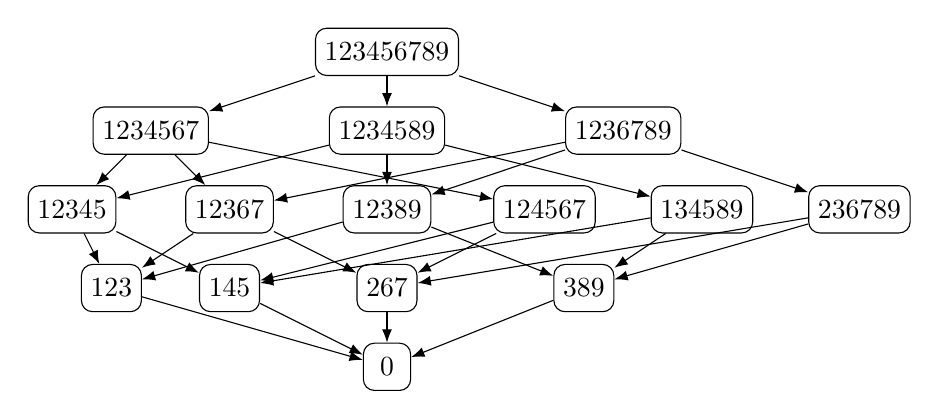
\begin{tikzpicture}[every node/.style={draw, rectangle, rounded corners, minimum size=6mm},
  ->, >=Latex, node distance=1cm]

% Level 1 (Top)
\node (A) at (0,4) {123456789};

% Level 2
\node (B1) at (-3,3) {1234567};
\node (B2) at (0,3)   {1234589};
\node (B3) at (3,3)   {1236789};

% Level 3
\node (C1) at (-4,2) {12345};
\node (C2) at (-2,2) {12367};
\node (C3) at (0,2)  {12389};
\node (C4) at (2,2)  {124567};
\node (C5) at (4,2)  {134589};
\node (C6) at (6,2)  {236789};

% Level 4
\node (D1) at (-3.5,1) {123};
\node (D2) at (-2,1)   {145};
\node (D3) at (0,1)    {267};
\node (D4) at (2.5,1)  {389};

% Level 5 (Bottom)
\node (O) at (0,0) {0};

% Edges from Top
\draw (A) -- (B1);
\draw (A) -- (B2);
\draw (A) -- (B3);

% Edges B1
\draw (B1) -- (C1);
\draw (B1) -- (C2);
\draw (B1) -- (C4);

% Edges B2
\draw (B2) -- (C1);
\draw (B2) -- (C3);
\draw (B2) -- (C5);

% Edges B3
\draw (B3) -- (C2);
\draw (B3) -- (C3);
\draw (B3) -- (C6);

% Edges C1
\draw (C1) -- (D1);
\draw (C1) -- (D2);

% Edges C2
\draw (C2) -- (D1);
\draw (C2) -- (D3);

% Edges C3
\draw (C3) -- (D1);
\draw (C3) -- (D4);

% Edges C4
\draw (C4) -- (D2);
\draw (C4) -- (D3);

% Edges C5
\draw (C5) -- (D2);
\draw (C5) -- (D4);

% Edges C6
\draw (C6) -- (D3);
\draw (C6) -- (D4);

% Edges to 0
\draw (D1) -- (O);
\draw (D2) -- (O);
\draw (D3) -- (O);
\draw (D4) -- (O);

\end{tikzpicture}
\end{center}
\end{proof}
 If we choose $x=123,y=267,z=389$ then \\
$2^n=8$ not hold
$x \vee(z \wedge y)\neq (x \vee y) \wedge (x \vee z) .$\\






\bigskip

 \begin{theorem}
     $lcm(I_H)$ is Boolean iff every $e\in H$ has a vertex $V_e$ s.t ${V_e \notin e^{'} \forall e^{'} \in E/e }$
\end{theorem}

\begin{proof}
  \textcolor{red}{\textbf{Proof 07}}
\end{proof}

\bigskip

\begin{corollary}
     If  $e\in H$ has a vertex $V_e$  such that ${V_e \notin e^{'} \forall e^{'} \in E/e }$ iff H does not contain any of the following.
   
     \begin{figure}[]
	\centering
	\includegraphics[width=8cm, height=5cm] 
         {boolean}\label{qwe}
	\caption{}.
     \end{figure}
\end{corollary}
    
\begin{proof}
  \textcolor{red}{\textbf{Proof 08}}
\end{proof}

\bigskip


\section*{Example: Non-Boolean LCM-Lattice from Triangle Graph}

Consider the graph \( G \) which is a triangle:

\begin{center}
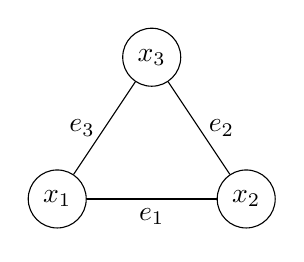
\begin{tikzpicture}[scale=1.2]
  \node[draw, circle] (a) at (0,0)  {$x_1$};
  \node[draw, circle] (b) at (2,0)  {$x_2$};
  \node[draw, circle] (c) at (1,1.5) {$x_3$};

  \draw (a) -- node[below]{$e_1$} (b);
  \draw (b) -- node[right]{$e_2$} (c);
  \draw (c) -- node[left]{$e_3$} (a);
\end{tikzpicture}
\end{center}

The edge ideal is:
\[
I(G) = (x_1x_2,\, x_2x_3,\, x_1x_3)
\]

The LCMs of subsets:
\begin{itemize}
    \item \( \mathrm{lcm}(x_1x_2, x_2x_3) = x_1x_2x_3 \)
    \item \( \mathrm{lcm}(x_1x_2, x_1x_3) = x_1x_2x_3 \)
    \item \( \mathrm{lcm}(x_2x_3, x_1x_3) = x_1x_2x_3 \)
    \item \( \mathrm{lcm}(x_1x_2, x_2x_3, x_1x_3) = x_1x_2x_3 \)
\end{itemize}

Observe: multiple different subsets have the same lcm \( x_1x_2x_3 \), so the mapping from subsets to lcm is not injective.

Hence, the LCM-lattice is not Boolean.

\textbf{Why?} Because subsets like:
\[
A = \{x_1x_2, x_2x_3\}, \quad B = \{x_1x_2, x_2x_3, x_1x_3\}
\]
have different sizes but give the same union of variables: \( \{x_1, x_2, x_3\} \), and thus same lcm.

\bigskip

\textbf{Conclusion:} This violates the condition in the theorem. Therefore, the LCM-lattice is not Boolean.
\newpage


\begin{remark}
An alternative approach considers the modularity of \({\LC}(I(G)) \) through monomial divisibility. Suppose \( x < y \) in the lattice, with \( x = \alpha_1 \alpha_2 \cdots \alpha_k \) and \( y = \alpha_1 \alpha_2 \cdots \alpha_k \beta_1 \beta_2 \cdots \beta_t \), where \(\alpha_i\) and \(\beta_j\) are variables from edge monomials, and let \( z = \gamma_1 \gamma_2 \cdots \gamma_k \). and 
     Since I(G) is modular and $x<y$.
      Suppose that ${\gamma_{i_{1}}} {\gamma_{i_{2}}}...{\gamma_{i_{t^{'}}}}= {\alpha _{i_{1}}}{\alpha _{i_2}}...{\alpha _{i_{t^{'}}}}$
      and ${\gamma_{j_{1}}} {\gamma_{j_{2}}}...{\gamma_{j_{t^{''}}}}= {\alpha _{j_{1}}}{\alpha _{j_2}},..,{\alpha _{j_{t^{''}}}}$\\
      We need to show that:
      $$   x  \vee  (z\wedge y)=(x  \vee  Z)\wedge y$$ \\
       $x  \vee  (z\wedge y)=x  \vee ({\gamma_{1}} {\gamma_{2}}...{\gamma_{k}} \wedge {\alpha _{1}}{\alpha _{2}}...{\alpha _{k}} {\beta _{1}}{\beta _{2}},..,{\beta _{t}})$
       $=x \vee {\alpha _{i_{1}}}{\alpha _{i_{t^{'}}}}{\beta _{j_{1}}}{\beta _{j_{2}}}...{\beta _{j_{t^{''}}}}$\\
       \begin{equation}\label{aa}
            x  \vee  (z\wedge y) = {\alpha _{1}}{\alpha _{2}}...{\alpha _{k}}{\beta _{1}}{\beta _{2}},.., {\beta _{t}}
      \end{equation}
      Now, \\
      $ (x \vee z) \wedge y=x  \vee ({\gamma_{1}} {\gamma_{2}}...{\gamma_{k}}) \wedge {\alpha _{1}}{\alpha _{2}}...{\alpha _{k}} {\beta _{1}}{\beta _{2}},..,{\beta _{t}}$\\
      $ (x \vee z) \wedge y=({\alpha _{1}}{\alpha _{2}}...{\alpha _{k}}{\gamma_{1}} {\gamma_{2}}...{\gamma_{k}})  \wedge {\alpha _{1}}{\alpha _{2}}...{\alpha _{k}} {\beta _{1}}{\beta _{2}},..,{\beta _{t}}$
      \begin{equation}\label{qqq}
          (x \vee z) \wedge y={\alpha _{1}}{\alpha _{2}}...{\alpha _{k}}{\beta _{j_{1}}}{\beta _{j_{2}}}...{\beta _{j_{t^{''}}}}
      \end{equation}
       Consistent under modularity from Equation \ref{aa} and \ref{qqq}.\\
\textbf{Conversely},\\ 
     suppose on the contrary that \( G \) has an induced path of length $3$ with edges $\{x_1 x_2, x_2 x_3, x_3 x_4\} \in I(G)$\\
      We claim that I(G) is a modular then $\LC(I(G))$ satisfy the modular property.\\ 
      For any $ x_i \leq x_j$, in lattice $\&$ for any $x_k, \LC(I_G) $ will not satisfy modular property so is a contradiction. 
\end{remark}

\begin{theorem}
     Let $I=I(G)$ be an edge ideal of graph G then
     $\lcm(I)$ is modular if and only if maximum components of $G$ are of the form of triangle or path of length $2$.
\end{theorem}
%\begin{proof}
    Contrary suppose that there exists a path of length $3$ i.e.,
    \begin{figure}[]
	\centering
	\includegraphics[width=8cm, height=5cm] 
         {lattice}
	\caption{}.
    \end{figure}
    for $x=12, y=123, z=34$ with $x\leq y$, we have
    $$
    \begin{aligned}
       & x \vee(z \wedge y)=(x \vee z) \wedge y . \\
       & 12 \vee(34 \wedge 123)=(12 \vee 34) \wedge 123 . \\
       & 12 \vee(0)=(1234) \wedge 123 . \\
       & 12 \neq 123 
       %\text {} 
    \end{aligned}
    $$
    Hence, $I(G)$ is  not modular for path length $\geq 3$ because path length $3$ is always embedded into path length $>3$. \\
\textbf{Conversally,} \\
    suppose that if a graph does not has maximum path length $\geq 3$ then we need to show that it is modular.\\
    Since a graph having maximum path length $2$ is always Boolean \\ $\Rightarrow$ and since every boolean lattice is modular so path length 2 is always Modular.\\
    Now, any cycle having length greater than and equal to $4$ contains a path of length 3 that is  not  modular. but triangle is a special case having path length $3$ that is modular.

\bigskip

\bigskip
\begin{theorem}
Let $I = I(G)$ be the edge ideal of a graph $G$. Then the lcm-lattice $\lcm(I)$ is modular if and only if every connected component of $G$ is either a triangle or a path of length at most $2$.
\end{theorem}

\begin{proof}
We first prove the forward direction. Suppose, for contradiction, that $G$ contains a path of length $3$, say with edges $\{1,2\}, \{2,3\}, \{3,4\}$. In the lcm-lattice, consider the monomials:
\[
x = 12,\quad y = 123,\quad z = 34,
\]
where each number denotes a variable, and the monomials represent lcm of edges. Clearly, \( x \leq y \). Then,
\[
\begin{aligned}
x \vee (y \wedge z) &= (x \vee z) \wedge y, \\
12 \vee (123 \wedge 34) &= (12 \vee 34) \wedge 123, \\
12 \vee (0) &= 1234 \wedge 123, \\
12 &= 123 \neq 12.
\end{aligned}
\]
This contradicts the modular identity, so the lattice is not modular. Since any path of length greater than 3 contains a subpath of length 3, such graphs also fail modularity.

\medskip

\noindent \textbf{Conversely}, suppose that every connected component of $G$ is either a triangle or a path of length at most $2$. We show that $\lcm(I)$ is modular.

- For a path of length $2$ (three vertices and two edges), it is known that the lcm-lattice is Boolean, and every Boolean lattice is modular.
- A triangle (a 3-cycle) is a special case where the lcm-lattice is also modular, even though it is not Boolean.
- Since the modularity property is preserved under disjoint unions of modular sublattices (i.e., for each connected component), the entire lattice is modular.

Hence, $\lcm(I)$ is modular if and only if every component of $G$ is either a triangle or a path of length at most $2$.
\end{proof}


\begin{figure}[]
	\centering
	\includegraphics[width=8cm, height=5cm] 
         {lattice}
	\caption{}.
    \end{figure}




    \begin{figure}[h]
\centering
\begin{minipage}{0.45\textwidth}
\centering
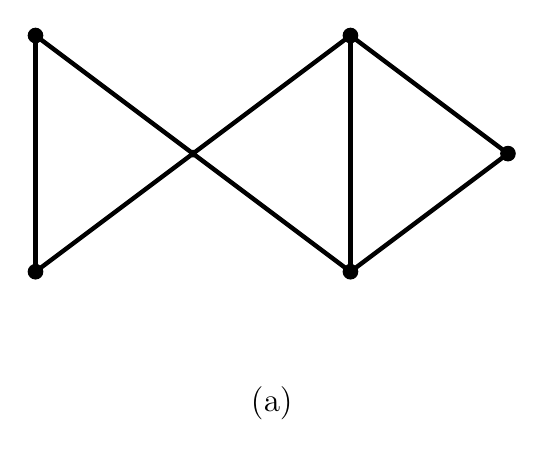
\begin{tikzpicture}[line join=round, line cap=round, scale=1]
  % styles
  \tikzset{
    v/.style={circle, fill=black, inner sep=2pt},   % main vertex
    vc/.style={circle, fill=black, inner sep=1pt}   % center vertex
  }

  % coordinates
  \coordinate (LT) at (0,1.5);   % left top
  \coordinate (LB) at (0,-1.5);  % left bottom
  \coordinate (C)  at (2,0);     % center
  \coordinate (MT) at (4,1.5);   % middle top
  \coordinate (MB) at (4,-1.5);  % middle bottom
  \coordinate (R)  at (6,0);     % right

  % edges
  \draw[line width=1.6pt] (LT) -- (LB);   % left vertical
  \draw[line width=1.6pt] (MT) -- (MB);   % middle vertical
  \draw[line width=1.6pt] (LT) -- (C);
  \draw[line width=1.6pt] (LB) -- (C);
  \draw[line width=1.6pt] (MT) -- (C);
  \draw[line width=1.6pt] (MB) -- (C);
  \draw[line width=1.6pt] (MT) -- (R);
  \draw[line width=1.6pt] (MB) -- (R);

  % vertices
  \node[v]  at (LT) {};
  \node[v]  at (LB) {};
  \node[vc] at (C)  {};
  \node[v]  at (MT) {};
  \node[v]  at (MB) {};
  \node[v]  at (R)  {};
  
  \node[below=18pt] at (3,-2.2) {\large (a)};
\end{tikzpicture}
\end{minipage}%
\hfill
\begin{minipage}{0.45\textwidth}
\centering
\begin{tikzpicture}[every node/.style={minimum size=6mm}, ->, >=Latex, scale=1]

% Level 1 (Top)
\node (A) at (0,4) {$x_1x_2x_3x_4x_5x_6$};

% Level 2
\node (B1) at (-2,3) {$x_1x_2x_3x_4$};
\node (B2) at (2,3)  {$x_2x_3x_4x_5x_6$};

% Level 3
\node (C1) at (-3,2) {$x_1x_2x_3$};
\node (C2) at (0,2)  {$x_2x_3x_4$};
\node (C3) at (3,2)  {$x_4x_5x_6$};

% Level 4 (Bottom)
\node (O) at (0,0) {$0$};

% Edges
\draw (A) -- (B1);
\draw (A) -- (B2);
\draw (B1) -- (C1);
\draw (B1) -- (C2);
\draw (B2) -- (C2);
\draw (B2) -- (C3);
\draw (C1) -- (O);
\draw (C2) -- (O);
\draw (C3) -- (O);

\node[below=18pt] at (0,-0.8) {\large (b)};
\end{tikzpicture}
\end{minipage}
\caption{(a) A hypergraph and (b) its corresponding $\operatorname{lcm}$-lattice.}
\end{figure}
\begin{theorem}\label{hypermodular}
     Let \( H = (V, E) \) be a \( k \)-uniform hypergraph, and let \( I(H) = (x_{i_1} \cdot \ldots \cdot x_{i_k} \mid \{i_1, \ldots, i_k\} \in E(H)) \) be its edge ideal, with \( L(I(H)) \) denoting its LCM lattice. Then the following are equivalent:
\begin{enumerate}
     \item[(a)] \( L(I(H)) \) is a modular lattice.
     \item[(b)] Every hyperedge \( e \in E(H) \) contains at least one vertex \( v_e \in e \) such that \( v_e \notin e' \) for all other hyperedges \( e' \in E(H) \setminus \{e\} \).
\end{enumerate}  
\end{theorem}
\begin{theorem}[]
     Let \( \H = (V, E) \) be a \(3\)-uniform hypergraph, and let \( I(
     \H) \) be its edge ideal with \(\LC(I(\H)) \) its LCM lattice. Then \(\LC(I(H)) \) is isomorphic to a Boolean lattice if and only if every hyperedge \( e \in E \) contains a \emph{unique vertex} \( v_e \in e \) such that \( v_e \notin e' \) for all other hyperedges \( e' \in E \setminus \{e\} \).
\end{theorem}


\begin{figure}
\centering
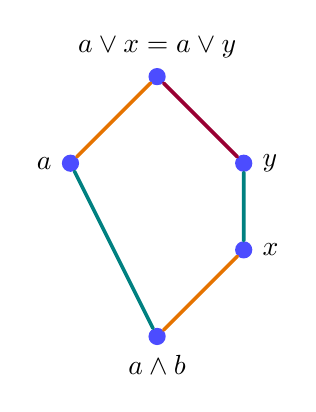
\begin{tikzpicture}[scale=1.1, line join=round, line cap=round]
  % styles
  \tikzset{
    v/.style={circle, fill=blue!70, inner sep=2.2pt, font=\small, text=white}, 
    edgea/.style={line width=1.3pt, teal},
    edgeb/.style={line width=1.3pt, orange!90!black},
    edgec/.style={line width=1.3pt, purple!80!black}
  }

  % vertices
  \node[v,label=above:{$a \vee x = a \vee y$}] (top) at (0,2) {};
  \node[v,label=left:{$a$}]   (a)   at (-1,1) {};
  \node[v,label=right:{$y$}]  (y)   at (1,1) {};
  \node[v,label=right:{$x$}]  (x)   at (1,0) {};
  \node[v,label=below:{$a \wedge b$}] (bot) at (0,-1) {};

  % edges with colors
  \draw[edgea] (bot)--(a);
  \draw[edgeb] (a)--(top);
  \draw[edgec] (top)--(y);
  \draw[edgea] (y)--(x);
  \draw[edgeb] (x)--(bot);

\end{tikzpicture}
\caption{}\label{FN5}
\end{figure}


\begin{theorem}
     Let $G$ be a graph, $I(G)$ be its edge ideal.  Let $\mathcal{L}=\lcm (I(G))$  be LCM  lattice of  $I(G)$. Then $\mathcal{L}$ is boolean if and only if  $E(G)$, the edge set of  $G$ does not contains two subsets $A$ and $B$, having different cardinality with    $${\cup}_{e \in B}=\cup_{e\in A}.$$
\end{theorem}
\begin{proof}
     Boolean lattice shows that a complete power set must be there at lcm lattice.\\
     Now, if $\exists$ a triangle having e-edges in which each edge is not sharing triangle then  if one define a bijection between $\lcm(H)$ and power set then there does not exist any element in $\lcm(H)$ which corresponds $e$.\\
     $ \Rightarrow e_1,e_2,e_3 \in E$ such that $e \in \cup _{i=1}^{3} {e_i}$ \\
     $ \Rightarrow e_1, e_2, e_3 \in E$ such that $e \in \cup_{i=1}^{3} {e_i} $
     $\Rightarrow $ a sublattice generated by $\cup_{i=1}^{3}{e_i}$ is not boolean.
\end{proof}




Proof for c) => a)
\textbf{\( c) \implies a) \)} \\
Assume for all \( A, B \subseteq E(H) \), if \( \bigcup_{e \in A} e = \bigcup_{e \in B} e \), then \( A = B \). Define \( f: \mathcal{P}(E(H)) \to \LC(I(H)) \) by \( A \mapsto \mathrm{lcm}(A) \). Since \( \bigcup_{e \in A} e = \bigcup_{e \in B} e \) implies \( A = B \), the map \( f \) is injective. As \( \mathcal{P}(E(H)) \) is finite and \( f \) maps to \( \LC(I(H)) \), which has \( |E(H)| \) atoms, \( f \) is also surjective. Thus, \( f \) is bijective, and since \( \mathcal{P}(E(H)) \) is a Boolean lattice, \( \LC(I(H)) \) is isomorphic to a Boolean lattice.






\begin{theorem}
      Let $H=(V,E)$ be a 3-uniform hypergraph then $\lcm(H) $is Boolean if and only f $H$ does not contain any of these (a) \& (b)
      see Figure \ref{aaas} 
      \begin{figure}[]\label{aaas}
	\centering
	\includegraphics[width=13cm, height=5cm]{hypergraphs}
	\caption{Hypergraphs}.
\end{figure}
  \begin{figure}[]
	    \centering
	      \includegraphics[width=14cm, height=5cm] 
          {hypergraph lattice}
	   \caption{Posets}.\label{012ee}
    \end{figure}

\end{theorem}

\bigskip


\begin{theorem}
    \textcolor{red}{Statement} \\ Let $H=(V,E)$ be a 3-uniform hypergraph, and I(H) be its edge ideal with \( \LC(I(H)) \) to be its LCM lattice. Then the following are equivalent.
\begin{itemize}
    \item[a)] $\LC (I(H))$ is isomorphic to a Boolean lattice,
    \item[b)] \( H \) contains no path of length $3$
    \end{itemize}
\end{theorem}
\begin{proof}
For (a):\\
if $x=123,y=234,z=456$ then \\
$2^n=8$ not hold
$x \vee(z \wedge y)\neq (x \vee y) \wedge (x \vee z) .$\\

\bigskip
For (b):\\
if $x=123,y=134,z=145$ then \\
$2^n=8$ not hold
$x \vee(z \wedge y)\neq (x \vee y) \wedge (x \vee z)  .$

Also distributive property does not hold for (c)
For (c):\\

\begin{center}
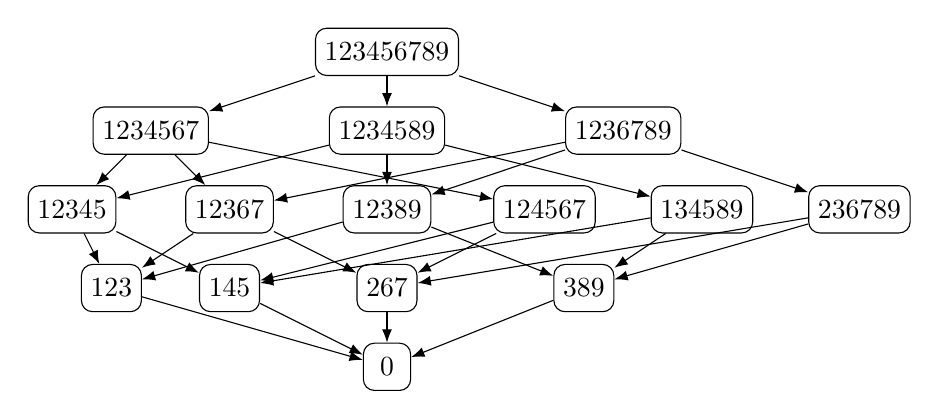
\begin{tikzpicture}[every node/.style={draw, rectangle, rounded corners, minimum size=6mm},
  ->, >=Latex, node distance=1cm]

% Level 1 (Top)
\node (A) at (0,4) {123456789};

% Level 2
\node (B1) at (-3,3) {1234567};
\node (B2) at (0,3)   {1234589};
\node (B3) at (3,3)   {1236789};

% Level 3
\node (C1) at (-4,2) {12345};
\node (C2) at (-2,2) {12367};
\node (C3) at (0,2)  {12389};
\node (C4) at (2,2)  {124567};
\node (C5) at (4,2)  {134589};
\node (C6) at (6,2)  {236789};

% Level 4
\node (D1) at (-3.5,1) {123};
\node (D2) at (-2,1)   {145};
\node (D3) at (0,1)    {267};
\node (D4) at (2.5,1)  {389};

% Level 5 (Bottom)
\node (O) at (0,0) {0};

% Edges from Top
\draw (A) -- (B1);
\draw (A) -- (B2);
\draw (A) -- (B3);

% Edges B1
\draw (B1) -- (C1);
\draw (B1) -- (C2);
\draw (B1) -- (C4);

% Edges B2
\draw (B2) -- (C1);
\draw (B2) -- (C3);
\draw (B2) -- (C5);

% Edges B3
\draw (B3) -- (C2);
\draw (B3) -- (C3);
\draw (B3) -- (C6);

% Edges C1
\draw (C1) -- (D1);
\draw (C1) -- (D2);

% Edges C2
\draw (C2) -- (D1);
\draw (C2) -- (D3);

% Edges C3
\draw (C3) -- (D1);
\draw (C3) -- (D4);

% Edges C4
\draw (C4) -- (D2);
\draw (C4) -- (D3);

% Edges C5
\draw (C5) -- (D2);
\draw (C5) -- (D4);

% Edges C6
\draw (C6) -- (D3);
\draw (C6) -- (D4);

% Edges to 0
\draw (D1) -- (O);
\draw (D2) -- (O);
\draw (D3) -- (O);
\draw (D4) -- (O);

\end{tikzpicture}
\end{center}
\end{proof}
 If we choose $x=123,y=267,z=389$ then \\
$2^n=8$ not hold
$x \vee(z \wedge y)\neq (x \vee y) \wedge (x \vee z) .$\\






\bigskip

 \begin{theorem}
     $lcm(I_H)$ is Boolean iff every $e\in H$ has a vertex $V_e$ s.t ${V_e \notin e^{'} \forall e^{'} \in E/e }$
\end{theorem}

\begin{proof}
  \textcolor{red}{\textbf{Proof 07}}
\end{proof}

\bigskip

\begin{corollary}
     If  $e\in H$ has a vertex $V_e$  such that ${V_e \notin e^{'} \forall e^{'} \in E/e }$ iff H does not contain any of the following.
   
     \begin{figure}[]
	\centering
	\includegraphics[width=8cm, height=5cm] 
         {boolean}\label{qwe}
	\caption{}.
     \end{figure}
\end{corollary}
    
\begin{proof}
  \textcolor{red}{\textbf{Proof 08}}
\end{proof}

\bigskip


\section*{Example: Non-Boolean LCM-Lattice from Triangle Graph}

Consider the graph \( G \) which is a triangle:

\begin{center}
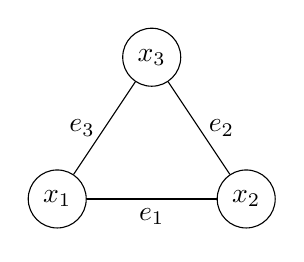
\begin{tikzpicture}[scale=1.2]
  \node[draw, circle] (a) at (0,0)  {$x_1$};
  \node[draw, circle] (b) at (2,0)  {$x_2$};
  \node[draw, circle] (c) at (1,1.5) {$x_3$};

  \draw (a) -- node[below]{$e_1$} (b);
  \draw (b) -- node[right]{$e_2$} (c);
  \draw (c) -- node[left]{$e_3$} (a);
\end{tikzpicture}
\end{center}

The edge ideal is:
\[
I(G) = (x_1x_2,\, x_2x_3,\, x_1x_3)
\]

The LCMs of subsets:
\begin{itemize}
    \item \( \mathrm{lcm}(x_1x_2, x_2x_3) = x_1x_2x_3 \)
    \item \( \mathrm{lcm}(x_1x_2, x_1x_3) = x_1x_2x_3 \)
    \item \( \mathrm{lcm}(x_2x_3, x_1x_3) = x_1x_2x_3 \)
    \item \( \mathrm{lcm}(x_1x_2, x_2x_3, x_1x_3) = x_1x_2x_3 \)
\end{itemize}

Observe: multiple different subsets have the same lcm \( x_1x_2x_3 \), so the mapping from subsets to lcm is not injective.

Hence, the LCM-lattice is not Boolean.

\textbf{Why?} Because subsets like:
\[
A = \{x_1x_2, x_2x_3\}, \quad B = \{x_1x_2, x_2x_3, x_1x_3\}
\]
have different sizes but give the same union of variables: \( \{x_1, x_2, x_3\} \), and thus same lcm.

\bigskip

\textbf{Conclusion:} This violates the condition in the theorem. Therefore, the LCM-lattice is not Boolean.
\newpage


\begin{remark}
An alternative approach considers the modularity of \({\LC}(I(G)) \) through monomial divisibility. Suppose \( x < y \) in the lattice, with \( x = \alpha_1 \alpha_2 \cdots \alpha_k \) and \( y = \alpha_1 \alpha_2 \cdots \alpha_k \beta_1 \beta_2 \cdots \beta_t \), where \(\alpha_i\) and \(\beta_j\) are variables from edge monomials, and let \( z = \gamma_1 \gamma_2 \cdots \gamma_k \). and 
     Since I(G) is modular and $x<y$.
      Suppose that ${\gamma_{i_{1}}} {\gamma_{i_{2}}}...{\gamma_{i_{t^{'}}}}= {\alpha _{i_{1}}}{\alpha _{i_2}}...{\alpha _{i_{t^{'}}}}$
      and ${\gamma_{j_{1}}} {\gamma_{j_{2}}}...{\gamma_{j_{t^{''}}}}= {\alpha _{j_{1}}}{\alpha _{j_2}},..,{\alpha _{j_{t^{''}}}}$\\
      We need to show that:
      $$   x  \vee  (z\wedge y)=(x  \vee  Z)\wedge y$$ \\
       $x  \vee  (z\wedge y)=x  \vee ({\gamma_{1}} {\gamma_{2}}...{\gamma_{k}} \wedge {\alpha _{1}}{\alpha _{2}}...{\alpha _{k}} {\beta _{1}}{\beta _{2}},..,{\beta _{t}})$
       $=x \vee {\alpha _{i_{1}}}{\alpha _{i_{t^{'}}}}{\beta _{j_{1}}}{\beta _{j_{2}}}...{\beta _{j_{t^{''}}}}$\\
       \begin{equation}\label{aa}
            x  \vee  (z\wedge y) = {\alpha _{1}}{\alpha _{2}}...{\alpha _{k}}{\beta _{1}}{\beta _{2}},.., {\beta _{t}}
      \end{equation}
      Now, \\
      $ (x \vee z) \wedge y=x  \vee ({\gamma_{1}} {\gamma_{2}}...{\gamma_{k}}) \wedge {\alpha _{1}}{\alpha _{2}}...{\alpha _{k}} {\beta _{1}}{\beta _{2}},..,{\beta _{t}}$\\
      $ (x \vee z) \wedge y=({\alpha _{1}}{\alpha _{2}}...{\alpha _{k}}{\gamma_{1}} {\gamma_{2}}...{\gamma_{k}})  \wedge {\alpha _{1}}{\alpha _{2}}...{\alpha _{k}} {\beta _{1}}{\beta _{2}},..,{\beta _{t}}$
      \begin{equation}\label{qqq}
          (x \vee z) \wedge y={\alpha _{1}}{\alpha _{2}}...{\alpha _{k}}{\beta _{j_{1}}}{\beta _{j_{2}}}...{\beta _{j_{t^{''}}}}
      \end{equation}
       Consistent under modularity from Equation \ref{aa} and \ref{qqq}.\\
\textbf{Conversely},\\ 
     suppose on the contrary that \( G \) has an induced path of length $3$ with edges $\{x_1 x_2, x_2 x_3, x_3 x_4\} \in I(G)$\\
      We claim that I(G) is a modular then $\LC(I(G))$ satisfy the modular property.\\ 
      For any $ x_i \leq x_j$, in lattice $\&$ for any $x_k, \LC(I_G) $ will not satisfy modular property so is a contradiction. 
\end{remark}

\begin{theorem}
     Let $I=I(G)$ be an edge ideal of graph G then
     $\lcm(I)$ is modular if and only if maximum components of $G$ are of the form of triangle or path of length $2$.
\end{theorem}
\begin{proof}
    Contrary suppose that there exists a path of length $3$ i.e.,
    \begin{figure}[]
	\centering
	\includegraphics[width=8cm, height=5cm] 
         {lattice}
	\caption{}.
    \end{figure}
    for $x=12, y=123, z=34$ with $x\leq y$, we have
    $$
    \begin{aligned}
       & x \vee(z \wedge y)=(x \vee z) \wedge y . \\
       & 12 \vee(34 \wedge 123)=(12 \vee 34) \wedge 123 . \\
       & 12 \vee(0)=(1234) \wedge 123 . \\
       & 12 \neq 123 
       %\text {} 
    \end{aligned}
    $$
    Hence, $I(G)$ is  not modular for path length $\geq 3$ because path length $3$ is always embedded into path length $>3$. \\
\textbf{Conversally,} \\
    suppose that if a graph does not has maximum path length $\geq 3$ then we need to show that it is modular.\\
    Since a graph having maximum path length $2$ is always Boolean \\ $\Rightarrow$ and since every boolean lattice is modular so path length 2 is always Modular.\\
    Now, any cycle having length greater than and equal to $4$ contains a path of length 3 that is  not  modular. but triangle is a special case having path length $3$ that is modular.
\end{proof}

\bigskip
\begin{theorem}
Let $I = I(G)$ be the edge ideal of a graph $G$. Then the lcm-lattice $\lcm(I)$ is modular if and only if every connected component of $G$ is either a triangle or a path of length at most $2$.
\end{theorem}

\begin{proof}
We first prove the forward direction. Suppose, for contradiction, that $G$ contains a path of length $3$, say with edges $\{1,2\}, \{2,3\}, \{3,4\}$. In the lcm-lattice, consider the monomials:
\[
x = 12,\quad y = 123,\quad z = 34,
\]
where each number denotes a variable, and the monomials represent lcm of edges. Clearly, \( x \leq y \). Then,
\[
\begin{aligned}
x \vee (y \wedge z) &= (x \vee z) \wedge y, \\
12 \vee (123 \wedge 34) &= (12 \vee 34) \wedge 123, \\
12 \vee (0) &= 1234 \wedge 123, \\
12 &= 123 \neq 12.
\end{aligned}
\]
This contradicts the modular identity, so the lattice is not modular. Since any path of length greater than 3 contains a subpath of length 3, such graphs also fail modularity.

\medskip

\noindent \textbf{Conversely}, suppose that every connected component of $G$ is either a triangle or a path of length at most $2$. We show that $\lcm(I)$ is modular.

- For a path of length $2$ (three vertices and two edges), it is known that the lcm-lattice is Boolean, and every Boolean lattice is modular.
- A triangle (a 3-cycle) is a special case where the lcm-lattice is also modular, even though it is not Boolean.
- Since the modularity property is preserved under disjoint unions of modular sublattices (i.e., for each connected component), the entire lattice is modular.

Hence, $\lcm(I)$ is modular if and only if every component of $G$ is either a triangle or a path of length at most $2$.
\end{proof}


Among these properties, modularity—characterized by the identity \( x \vee (y \wedge z) = (x \vee y) \wedge (x \vee z) \) for all elements \( x, y, z \) within the lattice—stands as a pivotal attribute, ensuring a harmonious interplay between join and meet operations. Complementing this, the Boolean structure, wherein the lattice is isomorphic to a power set lattice, imposes a total order that reflects the maximal combinatorial structure of the graph's edge set. On page 9, it is asserted that "The LCM-lattice of a graph \( G \) is Boolean if and only if \( G \) is a disjoint union of edges," a condition that ties the lattice's algebraic signature to the graph's decomposition into isolated pairs. This insight is further nuanced by the observation on the same page that "If \( G \) is connected and not a triangle, then the LCM-lattice of \( G \) is not Boolean," highlighting the restrictive nature of Booleanity in the presence of cycles or longer paths.



%see Figure \ref{aaas} 
   %   \begin{figure}[]\label{aaas}
	%\centering
	%\includegraphics[width=13cm, height=5cm]{hypergraphs}
%	\caption{Hypergraphs}.
%\end{figure}

%  \begin{figure}[]
%	    \centering
%	      \includegraphics[width=14cm, height=5cm] 
 %         {hypergraph lattice}
%	   \caption{Posets}.\label{012ee}
 %   \end{figure}


%%\end{proof}
%
%%\begin{theorem}\label{asd}
%%     Let $H=(V,E)$ be a $k$-uniform hypergraph, and let $I(H)=(x_i x_j x_k|\{i,j,k \} \in E) $ then $lcm(I(H))\cong Modular$ if and only if $H$ has no $3$-uniform hypergraph of the form (see Figure \ref{aaas}).
%     % of length $3$.
%%\end{theorem}
%
%\begin{proof}
%      Let a graph $I(H)$ be modular, and suppose on the contrary that there exists $3$-uniform hypergraph with path length $3$ having a connection of edges and vertices. Let $u,v,w$ be the set of atoms in $\lcm$-lattice where
%      $u=\{x_{i{_1}} {x_{i_2}} {x_{i_3}},
%      {x_{i_2}}{x_{i_3}{x_{i_4}}}, {x_{i_4}}
%      {x_{i_5}{x_{i_6}}}\},$v=
%      $\{x_{i{_1}}{x_{i_2}}x_{i_3},x_{i{_1}}{x_{i_3}}x_{i_4},x_{i{_1}}{x_{i_4}}x_{i_5}\}$, and $w=\{x_{i{_1}}{x_{i_2}}x_{i_3},x_{i{_3}}{x_{i_4}}x_{i_5},x_{i{_5}}{x_{i_6}}x_{i_7}\} \in E(I(G))$, (see Figure \ref{012ee}).
%%Since $\lcm$ of lattice of these elements is not modular.
%      Then for any $x,y \in \lcm$-lattice such that $x<y$ and for any $z \in \lcm$-lattice, %Since $\lcm$ of %these elements
%      $ \lcm(I(H))$ of  $u,v,w$ do not satisfy the modular property such that
%      $$x \vee(z \wedge y) \neq (x  \vee z) \wedge y, \ \  \ x<y.$$
%     %$\Rightarrow$
%      Hence, any% path of length $3$ or any
%      path embedded in the path of length $3$ with these shapes% $\lcm$-lattice with path length less than  $\exists$ is boolean and so
%      is not modular.
%
%\textbf{Conversally,}\\
%       Suppose that there  exists no $3$-uniform hypergraph. We need to show $\lcm$ lattice is modular. As we know that\ \ref{asd}, $\lcm$ lattice
%%of a graph $G$ having a path of length $< 3 $
% is always boolean if there exists no path of length $\geq 3$, and a boolean lattice is always modular so graph having no path of length $\geq 3$ is always modular. Hence,  $3$-uniform hypergraph having no path length $3$ is always modular.
%\end{proof}
%
%\bigskip
%
% \begin{corollary}
%     %  Let $G=(V,E)$ be a graph and $I(G)=(x_i x_j x_k|\{i,j,k \} \in E) $ then
%     If $lcm(I(G))\cong Modular$ then $G$ has no $3$-uniform hypergraph of the form \ref{aaas} if and only if $G$ is of path length less than equals to $3$.
%     % Figure \ref{aaas}.
%    % of length $3$.
% \end{corollary}
%
% \begin{proof}
%  \textcolor{red}{\textbf{Proof 09}}
% \end{proof}
%    for $x=12, y=123, z=34$ with $x\leq y$, we have
%    $$
%    \begin{aligned}
%       & x \vee(z \wedge y)=(x \vee z) \wedge y . \\
%       & 12 \vee(34 \wedge 123)=(12 \vee 34) \wedge 123 . \\
%       & 12 \vee(0)=(1234) \wedge 123 . \\
%       & 12 \neq 123
%       %\text {}
%    \end{aligned}
%    $$
%%%
